\documentclass[12pt]{scrartcl}
\usepackage[utf8x]{inputenc}
\usepackage{fullpage}

\usepackage{amsmath,mathtools}
\usepackage{amsfonts}
\usepackage{amssymb}
\usepackage{amsthm}
\usepackage{graphicx}
\usepackage{enumitem}
\usepackage[colorlinks=true, allcolors=blue]{hyperref}
\usepackage{mathrsfs}
\usepackage{bbm}
\usepackage{eucal,upgreek}
\usepackage{xcolor}

\usepackage{tikz}
\usetikzlibrary{arrows.meta,calc,positioning}

\usepackage[inline]{showlabels}
\renewcommand{\showlabelfont}{\tiny\ttfamily\color{gray}}

\renewcommand{\.}{\cdot}

\renewcommand{\b}{\mathbf{b}}
\renewcommand{\d}[1]{\mathrm{d}#1}
\newcommand{\tx}[1]{\text{#1}}
\newcommand{\up}[1]{\overline{#1}}
\newcommand{\lo}[1]{\underline{#1}}
\newcommand{\Ind}{\mathbbm{1}}
\renewcommand{\a}{\mathcal{B}}
\newcommand{\dnabla}{\overline{\nabla}}
\DeclareMathOperator*{\ddiv}{\overline{\mathsf{div}}}
\newcommand{\ent}{\textsf{Ent}}
\newcommand{\id}{\mathsf{id}}

\newcommand{\calAC}{\mathcal{AC}}
\newcommand{\calCc}{\mathcal{C}_c^\infty}
\newcommand{\calCb}[1]{\mathcal{C}_b(#1)}
\newcommand{\supp}{\text{supp}\,}
\newcommand{\leb}{\textsf{Leb}}

\newcommand{\dd}{\,\mathrm{d}}

\newcommand{\G}{\mathbf{G}}
\renewcommand{\v}{\mathbf{v}}
\newcommand{\V}{\mathbf{V}}
\newcommand{\e}{\mathbf{e}}
\newcommand{\x}{\mathbf{x}}
\newcommand{\p}{\mathbf{p}}
\renewcommand{\j}{\mathbf{j}}
\newcommand{\X}{\mathbf{X}}
\newcommand{\y}{\mathbf{y}}
\newcommand{\s}{\mathbf{s}}
\renewcommand{\r}{\mathbf{r}}
\renewcommand{\c}{\mathbf{c}}
\newcommand{\bxi}{\boldsymbol{\xi}}
\newcommand{\bpi}{\boldsymbol{\pi}}
\newcommand{\bvartheta}{\boldsymbol{\vartheta}}
\newcommand{\bsigma}{\boldsymbol{\sigma}}

\newcommand{\fra}{\mathfrak{a}}
\newcommand{\frA}{\mathfrak{A}}
\newcommand{\frC}{\mathfrak{C}}
\newcommand{\frD}{\mathfrak{D}}
\newcommand{\frE}{\mathfrak{E}}
\newcommand{\frF}{\mathfrak{F}}
\newcommand{\frG}{\mathfrak{G}}
\newcommand{\frh}{\mathfrak{h}}
\newcommand{\frH}{\mathfrak{H}}
\newcommand{\frl}{\mathfrak{l}}
\newcommand{\frm}{\mathfrak{m}}
\newcommand{\frs}{\mathfrak{s}}
\newcommand{\frX}{\mathfrak{X}}
\newcommand{\fru}{\mathfrak{u}}
\newcommand{\fry}{\mathfrak{y}}
\newcommand{\frY}{\mathfrak{Y}}
\newcommand{\frz}{\mathfrak{z}}
\newcommand{\frZ}{\mathfrak{Z}}
\newcommand{\frW}{\mathfrak{W}}

\newcommand{\calA}{\mathcal{A}}
\newcommand{\calB}{\mathcal{B}}
\newcommand{\calC}{\mathcal{C}}
\newcommand{\calD}{\mathcal{D}}
\newcommand{\calE}{\mathcal{E}}
\newcommand{\calF}{\mathcal{F}}
\newcommand{\calG}{\mathcal{G}}
\newcommand{\calH}{\mathcal{H}}
\newcommand{\calI}{\mathcal{I}}
\newcommand{\calJ}{\mathcal{J}}
\newcommand{\calK}{\mathcal{K}}
\newcommand{\calL}{\mathcal{L}}
\newcommand{\calM}{\mathcal{M}}
\newcommand{\calO}{\mathcal{O}}
\newcommand{\calP}{\mathcal{P}}
\newcommand{\calR}{\mathcal{R}}
\newcommand{\calV}{\mathcal{V}}
\newcommand{\calS}{\mathcal{S}}
\newcommand{\calU}{\mathcal{U}}
\newcommand{\calX}{\mathcal{X}}

\newcommand{\Diff}{\mathrm{D}}
\newcommand{\riesz}{I_\text{R}}

\newcommand{\scrA}{\mathscr{A}}
\newcommand{\scrO}{\mathscr{O}}
\newcommand{\scrP}{\mathscr{P}}
\newcommand{\scrS}{\mathscr{S}}
\newcommand{\scrN}{\mathscr{N}}
\newcommand{\scrU}{\mathscr{U}}

\newcommand{\bbC}{\mathbb{C}}
\newcommand{\bbE}{\mathbb{E}}
\newcommand{\bbF}{\mathbb{F}}
\newcommand{\bbG}{\mathbb{G}}
\newcommand{\bbI}{\mathbb{I}}
\newcommand{\bbK}{\mathbb{K}}
\newcommand{\bbP}{\mathbb{P}}
\newcommand{\bbN}{\mathbb{N}}
\newcommand{\bbR}{\mathbb{R}}
\newcommand{\bbS}{\mathbb{S}}
\newcommand{\bbT}{\mathbb{T}}
\newcommand{\bbW}{\mathbb{W}}
\newcommand{\bbZ}{\mathbb{Z}}

\newcommand{\sfa}{\mathsf{a}}
\newcommand{\sfA}{\mathsf{A}}
\renewcommand{\sfb}{\mathsf{b}}
\newcommand{\sfd}{\mathsf{d}}
\newcommand{\sfe}{\mathsf{e}}
\newcommand{\sfE}{\mathsf{E}}
\newcommand{\sfh}{\mathsf{h}}
\newcommand{\sfI}{\mathsf{I}}
\newcommand{\sfL}{\mathsf{L}}
\newcommand{\sfp}{\mathsf{p}}
\newcommand{\sfM}{\mathsf{M}}
\newcommand{\sfN}{\mathsf{N}}
\newcommand{\sfP}{\mathsf{P}}
\newcommand{\sfQ}{\mathsf{Q}}
\newcommand{\sfR}{\mathsf{R}}
\newcommand{\sfS}{\mathsf{S}}
\newcommand{\sfT}{\mathsf{T}}
\newcommand{\sfW}{\mathsf{W}}
\newcommand{\sfX}{\mathsf{X}}
\newcommand{\sfY}{\mathsf{Y}}
\newcommand{\sfZ}{\mathsf{Z}}

\newcommand{\rmI}{\mathrm{I}}

\newcommand{\dom}{\text{dom}\,}

\newcommand{\scrL}{\mathscr{L}}

\DeclareMathOperator*{\argmin}{\text{argmin}}
\DeclareMathOperator*{\tr}{\text{tr}}

\newcommand{\ket}[1]{\lvert #1 \rangle}
\newcommand{\bra}[1]{\langle #1 \rvert}
\newcommand{\braket}[2]{\langle #1 \!\mid\! #2 \rangle}
\newcommand{\oba}{\mathsf{a}}
\newcommand{\obb}{\mathsf{b}}

\newcommand{\alert}[1]{{\color{red}#1}}

%\newtheoremstyle{thmstyle}{}{}{\itshape}{}{\bfseries}{}{0.5em}{}
%\theoremstyle{thmstyle}
\newtheorem{theorem}{Theorem}[section]
\newtheorem{proposition}[theorem]{Proposition}
\newtheorem{lemma}[theorem]{Lemma}
\newtheorem{corollary}[theorem]{Corollary}

\newtheoremstyle{notestyle}{}{}{}{}{\bfseries}{}{0.5em}{}
\theoremstyle{notestyle}
\newtheorem{definition}[theorem]{Definition}
\newtheorem{exercise}{Exercise}[section]
\newtheorem{remark}[theorem]{Remark}
\newtheorem{example}[theorem]{Example}

\numberwithin{equation}{section}

\title{\LARGE Gradient Structures\\ from Classical to Quantum\\[0.8em]}
\author{Oliver Tse \\ {\normalsize Eindhoven University of Technology}}
\date{\small Updated on \today}



\begin{document}
\maketitle

\vspace{-4em}
\begin{center}\footnotesize
	Tutorial notes given at IPAM in Spring 2025
\end{center}


\begin{abstract} \small
	\noindent{\em Abstract.} 
\end{abstract}

% \setcounter{tocdepth}{1}

\vspace{-1em}
 \tableofcontents
 \thispagestyle{empty}

\newpage

\setcounter{page}{1}

%%\section{Quantum measurement processes}
\section{Stochastic Schr\"odinger Equation}

As we have seen, a quantum circuit is essentially a noisy controlled Schr\"odinger equation. In this section, we consider classical noise sources arising from the control mechanism in terms of light-matter interactions. Without going into the details of the physics, we introduce the stochastic Schr\"odinger equation, which captures the evolution of a quantum system driven by classical noise sources.

Let $\calH$ be a Hilbert space and $\scrB(\calH)$ be the space of bounded operators on $\calH$. We also consider the following subspaces of $\scrB(\calH)$ that play a distinguishing role:
\begin{align*}
	\scrU(\calH) &:= \bigl\{ \oba\in \scrB(\calH) : \oba^\dagger \oba = \sfI_\calH \bigr\} &\text{(unitary operators)}\\
	\scrO(\calH) &:= \bigl\{ \oba\in \scrB(\calH) : \oba^\dagger = \oba \bigr\} &\text{(hermitian operators)}
\end{align*}
where $\oba^\dagger \coloneqq \overline\oba^\top$ is the hermitian conjugate of an operator $\oba\in \scrB(\calH)$. 

Given a Hamiltonian $H\in\scrO(\calH)$ and a real-valued smooth path $\alpha_t$, the Schr\"odinger equation driven by $\dot\alpha_t H$ may be expressed as an evolution in the space $\scrU(\calH)$:
\[
	\d U_t = iHU_t\dd \alpha_t,\qquad U_0 = \sfI_\calH.
\]
In particular, the solution may be explicitly expressed as
\[
	U_t = \exp\bigl(i(\alpha_t-\alpha_0) H\bigr)\sfI_\calH.
\]
In the presence of noise, however, $\alpha_t$ is no longer smooth. Yet, if 
\[
	\alpha_t = \alpha_0 + B_t + M_t,
\]



\begin{align*}
	\d U_t = HU_t\,\d t + \sum\nolimits_j V_jU_t\circ \d\alpha_t,
\end{align*}
where $H$, $V_j$ are 




\subsection{Quantum measurements}

Let $\varrho\in\calS(\calH)$ be a state on a Hilbert space $\calH$ and $t\mapsto U_t \in \calU(\calH)$ be a group of unitary actions on $\calH$. Suppose $\sfQ$ is an $\bbR$-valued observable with spectral measure $\pi^\sfQ:\calB(\bbR)\to \calP(\calH)$, i.e., $\pi^\sfQ$ is a projection-valued measure (PVM). Then the probability of measuring an event $A\in\calB(\bbR)$ at time $t^->0$ is given by Born's rule:
\[
	\bbP_\varrho(\lambda_{t^-}^\sfQ\in A) = \tr[\pi^\sfQ(A)\varrho_{t^-}] = \tr[U_t^\dagger\pi^\sfQ(A)U_t \varrho]. 
\]
As measurements generally change the state of the system, L\"uders' rule postulates that, \emph{conditioned} on the event $A\in \calB(\bbR)$, the state ``collapses" to
\[
	\varrho_{t^+} = \scrS(\pi^\sfQ(A),\varrho_{t^-}),\qquad \scrS(\pi,\varrho) \coloneqq \frac{\pi\varrho\,\pi^\dagger}{\tr[\pi\varrho \pi^\dagger]}\in\calS(\calH).
\]
Notice that by definition, $\scrS(\pi,U\varrho\,U^\dagger) = \scrS(\pi U,\varrho)$ and $U\scrS(\pi,\varrho) U^\dagger=\scrS(U\pi,\varrho)$.

The probability of measuring the event $B\in\calB(\bbR)$ at time $t^+>0$ given that the event $A\in\calB(\bbR)$ was measured at time $t>0$ is
\[
	\bbP_\varrho(\lambda_{t^+}^\sfQ\in B\,|\,\lambda_{t^-}^\sfQ\in A) = \tr[\pi^\sfQ(B)\scrS(\pi^\sfQ(A),\varrho_{t^-})] = \frac{\tr[\pi^\sfQ(A\cap B)\varrho_{t^-}]}{\tr[\pi^\sfQ(A)\varrho_{t^-}]}.
\]
In particular, the conditional probability of measuring event $A\in\calB(\bbR)$ at time $t^+>0$ given it was measured at time $t^->0$ is $1$. If $\sfR$ is another $\bbR$-valued observable, then
\[
	\bbP_\varrho(\lambda_{t^+}^\sfR\in B\,|\,\lambda_{t^-}^\sfQ\in A) = \tr[\pi^\sfR(B)\varrho_{t^+}] = \frac{\tr[\pi^\sfR(B)\pi^\sfQ(A)\varrho_{t^-}\pi^\sfQ(A)\pi^\sfR(B)]}{\tr[\pi^\sfQ(A)\varrho_{t^-}]}.
\]
When $\sfR$ and $\sfQ$ commute, then $\pi^\sfR(B)\pi^\sfQ(A) = \pi^\sfQ(A)\pi^\sfR(B)$, and hence,
\[
	\bbP_\varrho(\lambda_{t^+}^\sfR\in B\,|\,\lambda_{t^-}^\sfQ\in A)\bbP_\varrho(\lambda_{t^-}^\sfQ\in A) = \bbP_\varrho(\lambda_{t^+}^\sfQ\in A\,|\,\lambda_{t^-}^\sfR\in B)\bbP_\varrho(\lambda_{t^-}^\sfR\in B),
\]
i.e., Bayes' theorem holds and the usual notion of joint probability is well defined. Clearly, this does not hold when $\sfR$ and $\sfQ$ do not commute. It is this failure of the Bayes theorem that distinguishes quantum probability from classical probability. 

In a similar fashion, one determines the probability of measuring the event $A_2$ at time $t_2^->0$ for $\sfR$ given that the event $A_1$ was measured at time $t_1>0$ for $\sfQ$ from 
\begin{align*}
	\bbP_\varrho(\lambda_{t_2^-}^\sfR\in A_2\,|\,\lambda_{t_1^-}^\sfQ\in A_1) 
	%&= \tr[\pi^\sfR(A_2)\varrho_{t_2^-}],\qquad \varrho_{t_2^-} = U_{t_2-t_1}\scrS(\pi^\sfQ(A_1),\varrho_{t_1^-})U_{t_2-t_1}^\dagger \\
%	&= \tr[\pi^\sfR(A_2)U_{t_2-t_1}\varrho_{t_1^+}U_{t_2-t_1}^\dagger] \\
	&= \tr[\pi^\sfR(A_2)U_{t_2-t_1}\scrS(\pi^\sfQ(A_1),\varrho_{t_1^-})U_{t_2-t_1}^\dagger] \\
%	&= \frac{\tr[\pi^\sfR(A_2)U_{t_2-t_1}\pi^\sfQ(A_1)U_{t_1}\varrho\, U_{t_1}^\dagger\pi^\sfQ(A_1)U_{t_2-t_1}^\dagger]}{\tr[\pi^\sfQ(A_1)U_{t_1}\varrho U_{t_1}^\dagger]} \\
	&= \tr[\pi^\sfR(A_2)U_{t_2-t_1} \scrS(\pi^\sfQ(A_1)U_{t_1},\varrho\, )U_{t_2-t_1}^\dagger] \\
	&= \tr[\pi^\sfR(A_2)\scrS(U_{t_2-t_1}\pi^\sfQ(A_1) U_{t_1}, \varrho)] = \tr[\pi^\sfR(A_2)\varrho_{t_2^-}].
\end{align*}
As before, upon measuring the event $A_2$ at time $t_2>0$, L\"uders' rule implies
\[
	\varrho_{t_2^+} = \scrS(\pi^\sfR(A_2),\varrho_{t_2^-}) = \scrS(\pi^\sfR(A_2)U_{t_2-t_1}\pi^\sfQ(A_1) U_{t_1},\varrho).
\]
Restricting ourselves to a single observable $\sfQ$, 


\section{Noncommutative probability}


\subsection{From commutative to noncommutative}

Consider the Hilbert space $\calH=L_\bbC^2(\Omega,\mu)$ over the complete probability space $(\Omega,\calF,\mu)$. Then any function $f\in L_\bbC^\infty(\Omega,\mu)$ gives rise to a multiplication operator $\sfM_f\in \calB(\calH)$:
\[
	\sfM_f \,g = fg \in \calH\qquad\forall\,g\in\calH,
\]
with $\|\sfM_f\|_\infty = \|f\|_{L^\infty(\mu)}$. The collection of all such multiplication operators
\[
	\scrA := \bigl\{ \sfM_f:f\in L_\bbC^\infty(\Omega,\mu) \bigr\}\subset\calB(\calH)
\]
forms a \emph{commutative} subalgebra of $\calB(\calH)$. 

\medskip
In fact, this subalgebra is a possibly noncommutative \emph{von Neumann} algebra:

\begin{definition}[von Neumann algebra]
	A (unital) \emph{von Neumann algebra} is a $*$-subalgebra $\scrA\subset \calB(\calH)$ that contains $I_\calH$ and is closed in the \emph{weak operator topology} (\textsc{wot}), i.e.,
	\[
		\textsc{wot-\!}\lim \oba_n = \oba\quad\Longleftrightarrow\quad \langle f,\oba_ng\rangle_\calH \to \langle f,\oba g\rangle_\calH\quad\forall f,g\in\calH.
	\]
	Equivalently, is it a $C^*$-algebra with a predual $\scrA_*$ that is a Banach space.
\end{definition}

There are sub-families of $\scrA$ that play a distinguished role, namely,
\begin{align*}
	\scrA_+ &:= \bigl\{ \oba\in \scrA : \oba\succeq 0 \bigr\} &\text{(nonnegative operators)}\\
	\scrO &:= \bigl\{ \oba\in \scrA : \oba^\dagger = \oba \bigr\} &\text{(Hermitian operators)} \\
	\scrP &:= \bigl\{ \oba\in \calO : \oba^2 = \oba \bigr\} &\text{(projection operators)}
\end{align*}
Here, $\oba\succeq 0$ if and only if $\langle f,\oba f\rangle_\calH\ge 0$ for all $f\in\calH$. Additionally, for von Neumann algebras, we also have the following useful density result:

\begin{proposition}
	Let $\scrA$ be a von Neumann algebra. Then 
	\[
		\scrA = \overline{\text{span}\,(\scrP)}^{\textsc{wot}},
	\]
	i.e., $\scrA$ is the \textsc{wot}-closure of the linear span of its projections.
\end{proposition}

Let us return to our previous example with $\scrA=\{ \sfM_f:f\in L_\bbC^\infty(\Omega,\mu)\}$. It is not difficult to see that $\scrA$ is a $W^*$-algebra. Notice that since $\sfM_f$ is self-adjoint for $f\in L_\bbR^\infty(\Omega,\mu)$, the family of self-adjoint operators is given by $\scrO=\{\sfM_f: f\in L_\bbR^\infty(\Omega,\mu)\}$ and the family of projection operators is given by $\scrP = \{\sfM_f\in\scrO : f=\mathbf{1}_A,\,A\in\calF\}$. 

\medskip
On a von Neumann algebra $\scrA$, we can talk about special types of continuous linear functionals on $\scrA$, called states.

\begin{definition}
	A \emph{state} on a von Neumann algebra $\scrA$ is a linear functional $\uppsi:\scrA\to \bbC$ that is positive and normalized, i.e., $\uppsi(\oba^\dagger \oba)\ge 0$ for all $\oba\in\scrA$ and $\uppsi(I_{\calB(\calH)})=1$.
	
	A state $\uppsi$ is said to be
	\begin{itemize}[itemsep=0.1em]
		\item[] \emph{faithful} if $\uppsi(\oba^\dagger \oba)=0\;\Leftrightarrow\; \oba=0$,
		\item[] \emph{tracial} if $\uppsi(\oba \obb)=\uppsi(\obb \oba)$ for all $\oba,\obb\in\scrA$, and
		\item[] \emph{normal} if $\uppsi\in\scrA_*$, i.e., if it is an element of the predual $\scrA_*$.
	\end{itemize}
\end{definition}



For any probability measure $\nu \ll \mu$, we set
\[
	\uppsi_\nu(\sfM_f) := \int_\Omega f \dd\nu,\qquad f\in L_\bbC^\infty(\Omega,\mu),
\]
we find that $\uppsi$ is a linear functional that is positive and normalized, i.e., $\uppsi$ is a state. Moreover, it is tracial. It is normal if $\omega:=d\nu/d\mu \in L^1(\Omega,\mu)$ and faithful if $\omega>0$.

\medskip
Normal states play an essential role, serving as a counterpart to classical measures, as made explicit by the following proposition.

\begin{proposition}\label{prop:normal-state}
	Let $\uppsi$ be a state on a von Neumann algebra $\scrA$. The following are equivalent:
	\begin{enumerate}[label=(\roman*),itemsep=0.1em]
		\item $\uppsi$ is a normal state.
		\item ($\sigma$-additivity) If $(\oba_n)\subset\calP$ are mutually orthogonal projections, i.e., $\oba_n(\calH)\perp \oba_m(\calH)$ for all $n\ne m$, and $\oba=\vee_n\, \oba_n$ being the projection on the smallest closed subspace containing $\cup_n\, \oba_n(\calH)$, then
		\[
			\uppsi(\oba) = \sum\nolimits_n \uppsi(\oba_n).
		\]
		\item (Continuity from below) For any increasing net $0\preceq \oba_n \uparrow \oba$ in $\scrA_+$, one has the increasing limit $\uppsi(\oba_n)\uparrow\uppsi(\oba)$.
		\item There exists a family $\{\xi_n\}\subset\calH$ with $\sum_n \|\xi_n\|_\calH^2 = 1$ such that\footnote{[Theorem 7.1.8, Fundamentals of the Theory of Operator Algebras, V.II, Kadison-Ringrose]}
		\[
			\uppsi = \sum\nolimits_n \langle \xi_n,\cdot\, \xi_n\rangle\qquad\text{in the sense of norm convergence}.
		\]
	\end{enumerate}
\end{proposition}

%\begin{definition}
%		A von Neumann algebra $\scrA$ is said to be \emph{$\sigma$-finite} if it admits at most countably many orthogonal projections.
%\end{definition}
%
%\begin{proposition}
%	Let $\scrA$ be a von Neumann algebra. Then the following are equivalent:
%	\begin{enumerate}[label=(\roman*),itemsep=0.1em]
%		\item $\scrA$ is $\sigma$-finite.
%		\item There exists a countable separating subset of $\calH$ for $\scrA$.
%		\item There exists a faithful positive linear functional in $\scrA_*$.
%	\end{enumerate}
%\end{proposition}


Consider an arbitrary normal state $\uppsi$ and set
\[
	\mu(A) := \uppsi(\sfM_{\mathbf{1}_A})\qquad\text{for every $A\in\calF$}.
\]
Then, clearly, $\mu(\emptyset)=0$, $\mu(\Omega)=\uppsi(I_{\calB(\calH)})=1$ and $\mu$ is $\sigma$-additive due to the equivalent characterization of a normal state given by Proposition~\ref{prop:normal-state}(ii). In particular, one obtains a classical measure on $(\Omega,\calF)$. In this sense, a state on a noncommutative von Neumann algebra generalizes that of a classical measure.

%\medskip
%Along this line of thought, one could define a probability distribution on $\scrP$ analogously. Indeed, for a normal state $\uppsi$ on a von Neumann algebra $\scrA$, one sets
%\[
%	\mu(a)=\uppsi(a)\qquad\forall\,a\in\scrP.
%\]
%If $\chi_\mu(\psi):=\mu(|\psi\rangle\langle \psi|)$ where $\|\psi\|_\calH=1$, then $\chi_\mu(c\psi)=\chi_\mu(\psi)$ for any $c\in\bbC$ with $|c|=1$. Moreover, for any orthonormal basis $\{\psi_j\}\subset\calH$, we have that $\sum_j |\psi_j\rangle\langle \psi_j| = I_\calH$, and thus $\sum_j \chi_\mu(\psi_j)=1$. Gleason's theorem\footnote{Parthasarathy} states that for Hilbert spaces with dimension $d\ge 3$, there exists a bounded operator $T_\mu$ on $\calH$ such that $\chi_\mu(\psi)=\langle \psi,T_\mu\psi\rangle$ for all $\|\psi\|=1$. 
%
%\begin{proposition}
%	Let $\mu$ be a probability distribution on $\scrP$, where $\dim\calH\ge 3$. Then there exists an orthonormal set $\{\psi_j\}\subset\calH$ and positive scalars $\{p_j\}$ with $\sum_j p_j=1$ such that
%	\[
%		\mu(a) = \sum\nolimits_j p_j \langle\psi_j,a\psi_j\rangle\qquad\forall\,a\in\scrP
%	\]
%\end{proposition}

\subsection{Observables}

In classical probability, we are often interested in computing expressions like $\bbP(X\in A)$, where $X$ is a random variable and $A\subset\bbR$ is a Borel set. 

In the quantum world, a random variable is modelled by a Hermitian operator $\oba\in\scrO$ and is called an \emph{observable}. Observables have their spectrum in $\bbR$ and can therefore be \emph{measured}.

Given a $\uppsi$ on a von Neumann algebra $\scrA$, the expectation of an observable $\oba$ w.r.t.\ the state $\uppsi$ is given by $\uppsi(\oba)$. Since every observable $\oba\in\scrO$ has a spectral decomposition
\[
	\oba = \int_\bbR \lambda\, E_\oba(d\lambda),\qquad E_\oba \,\widehat{=}\, \text{$\scrP$-valued measure,}
\]
we can associate a classical probability measure with the observable $\oba$ and state $\uppsi$:
\[
	\bbP_\uppsi(\oba\in A) := \uppsi(E_\oba(A))\qquad\text{for all Borel set $A\subset\bbR$}.
\]
For two observables $\oba,\obb\in\scrO$ that do not commute, one would like to be able to write $\bbP_\uppsi(\oba\in A,\obb\in B)$ for two Borel sets $A,B\subset\bbR$. The simple argument for this is that if $[\oba,\obb]\ne 0$, then $E_\oba(A)$ and $E_\obb(B)$ may not commute for all Borel sets $A, B$. In particular, 
\[
	\uppsi(E_\oba(A)E_\obb(B)) \ne \uppsi(E_\obb(B)E_\oba(A)),
\]
so there is no consistent way of writing $\bbP_\uppsi(\oba\in A,\obb\in B)$. Yet, when they do commute, then $\uppsi(E_\oba(A)E_\obb(B))=\uppsi(E_\obb(B)E_\oba(A))$ and a joint distribution exists and we are back to the classical scenario. 

\medskip
However, this turns out not to be possible, as the following example portrays.


\begin{example}[Stern-Gerlach measurements] 

Take a beam of atoms (each with spin-$\tfrac{1}{2}$) and perform the following steps:
\begin{figure}[h]\centering
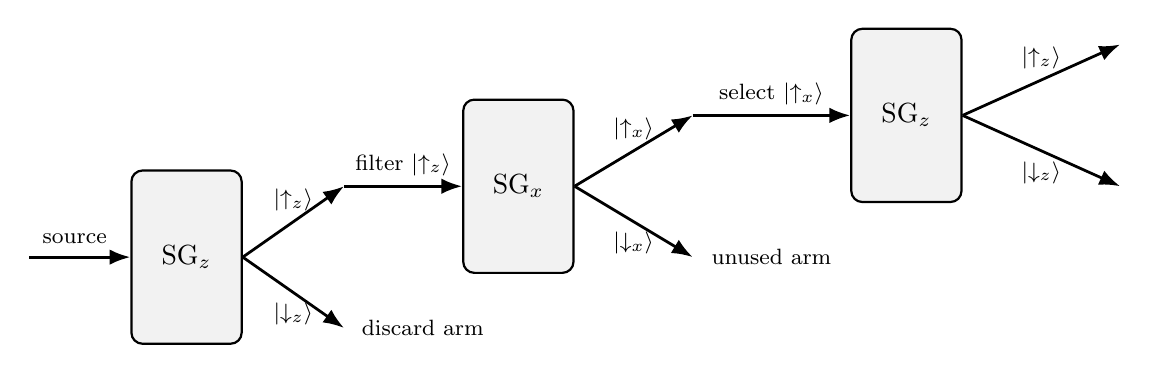
\begin{tikzpicture}[
    >=Latex,
    beam/.style={line width=1.0pt},
    magnet/.style={draw,rounded corners,minimum width=14mm,minimum height=22mm,thick,align=center,fill=gray!10},
    block/.style={draw,thick,minimum width=10mm,minimum height=6mm,fill=red!10,align=center},
%    det/.style={draw,thick,circle,minimum size=3mm,fill=black!70},
    note/.style={font=\footnotesize}
]

% --- Positions ---
% Source and first SG_z
\coordinate (S) at (-2,0);
\node[magnet] (SGz1) at (0,0) {SG$_z$};

% After SGz1 split
\coordinate (zup)   at (2, 0.9);
\coordinate (zdown) at (2,-0.9);

% Block on the down arm
\node[note] (Blk) at ($(zdown)+(1,0)$) {discard arm};

% SG_x on the up arm
\node[magnet,right=1.5cm of zup] (SGx) {SG$_x$};

% After SGx split
\coordinate (xup)   at ($(SGx.east)+(1.5, 0.9)$);
\coordinate (xdown) at ($(SGx.east)+(1.5,-0.9)$);

% Choose the +x branch into final SG_z
\node[magnet,right=2.0cm of xup] (SGz2) {SG$_z$};

% After SGz2 split
\coordinate (zup2)   at ($(SGz2.east)+(2.0, 0.9)$);
\coordinate (zdown2) at ($(SGz2.east)+(2.0,-0.9)$);

% --- Beams ---

% Source to first SG_z
\draw[beam,->] (S) -- (SGz1.west) node[pos=0.9,above left=1pt and 1pt,note] {source};

% SG_z split
\draw[beam,->] (SGz1.east) -- (zup)   node[midway,above,note] {$\ket{\uparrow_z}$};
\draw[beam,->] (SGz1.east) -- (zdown) node[midway,below,note] {$\ket{\downarrow_z}$};

% Block the down arm
%\draw[beam] (zdown) -- (Blk.west);
%\draw[very thick] ($(Blk.north west)+(0.5mm,0)$) -- ($(Blk.south east)+(-0.5mm,0)$);
%\draw[very thick] ($(Blk.south west)+(0.5mm,0)$) -- ($(Blk.north east)+(-0.5mm,0)$);

% Up arm into SG_x
\draw[beam,->] (zup) -- (SGx.west) node[midway,above,note] {filter $\ket{\uparrow_z}$};

% SG_x split (50/50)
\draw[beam,->] (SGx.east) -- (xup)   node[midway,above,note] {$\ket{\uparrow_x}$ };
\draw[beam,->] (SGx.east) -- (xdown) node[midway,below,note] {$\ket{\downarrow_x}$};

% Route +x arm to final SG_z
\draw[beam,->] (xup) -- (SGz2.west) node[midway,above,note] {select $\ket{\uparrow_x}$};

% Final SG_z split (50/50 again)
\draw[beam,->] (SGz2.east) -- (zup2)   node[midway,above,note] {$\ket{\uparrow_z}$};
\draw[beam,->] (SGz2.east) -- (zdown2) node[midway,below,note] {$\ket{\downarrow_z}$};

% Detectors (optional)
%\node[det] at (zup2) {};
%\node[det] at (zdown2) {};
%\node[det] at (xdown) {};

% Labels on devices
%\node[note,below=2mm of SGz1] {measure $z$};
%\node[note,below=2mm of SGx]  {measure $x$};
%\node[note,below=2mm of SGz2] {measure $z$};

% Explanatory notes
%\node[note,below right=1mm and -2mm of zdown] {discard arm};
\node[note] at ($(xdown)+(1,0)$) {unused arm};
\end{tikzpicture}
\caption{Stern-Gerlach experiment}
\end{figure}


\begin{enumerate}
	\item[\textbf{SG$_z$}] Measure spin in $z$-direction: Send the beam through a Stern-Gerlach magnet oriented along $z$. The beam splits into spin-up $\ket{\uparrow}$ and spin-down $\ket{\uparrow}$ paths. Keep only the spin-up branch, which gives a pure state $\ket{\uparrow_z}$.

	\item[\textbf{SG$_x$}] Measure spin in $x$-direction: Now send the filtered beam through a second magnet, oriented along $x$. The beam splits again into $\ket{\uparrow_x}$ and $\ket{\downarrow_x}$ outcomes with $50\%$--$50\%$ probability. So far, this can \emph{still} be explained with classical probability.
	
	\item[\textbf{SG$_z$}] Measure spin in $z$-direction again: Send either of the filtered beams $\ket{\uparrow_x}$ or $\ket{\downarrow_x}$ through a $z$-magnet again. You do \emph{not} get back the original result, i.e., instead of remaining spin-up, you see another $50\%$--$50\%$ split between $\ket{\uparrow_z}$ and $\ket{\downarrow_z}$
\end{enumerate}

Morally, if spin-$x$ and spin-$z$ were classical random variables, measuring $x$ would \emph{erase} knowledge of $z$. In classical probability, observing one property never randomizes another unless there is \emph{hidden causal disturbance}.

Quantum mechanically, the two observables (or random variables)
\begin{align*}
	\sigma_z = \begin{bmatrix}
		1 & 0 \\ 0 &-1
	\end{bmatrix}\quad\text{spin in $z$-direction},\qquad 
	\sigma_x = \begin{bmatrix}
		0 & 1 \\ 1 &0
	\end{bmatrix}\quad\text{spin in $x$-direction}.
\end{align*}
do not commute, i.e., $[\sigma_x,\sigma_y]\ne 0$, and measuring $\sigma_x$ \emph{changes} information about $\sigma_z$. In this sense, they cannot be jointly sampled, i.e., there is no classical joint probability $p(\sigma_x,\sigma_z)$ for these observables, which illustrates the need for noncommutative probability.
\end{example}








\newpage
\section{Stochastic Dilation}



\subsection{Noncommutative random variables}

\begin{definition}\label{def:random-variable}
	A \emph{noncommutative $\frX$-valued random variable} on a quantum probability space $(\frA,\mu)$ is an identity preserving $*$-homomorphism
	\[
		\frz\colon \frX\to\frA.
	\]
	Correspondingly, a \emph{noncommutative $\frX$-valued stochastic process} on a quantum probability space $(\frA,\mu)$ is a family of random variables
	\[
		\frz_t\colon \frX\to \frA,\quad t\in\bbT,
	\]
	with $\bbT$ being a (possibly uncountable) index set.
\end{definition}

\begin{example}[Classical random variable]
	Let $X$ be a classical $E$-valued random variable on $(\Omega,\bbP)$. Setting
\[
	\frX\coloneqq B_b(E),\qquad \frA\coloneqq L^\infty(\Omega,\bbP),\qquad \mu(g)\coloneqq \int_\Omega g\dd\bbP,\quad g\in\frA,
\]
we have that
\[
		\frX\ni f\mapsto \frz(f) \coloneqq f\circ X \in L^\infty(\Omega,\bbP)
\]
is a noncommutative $\frX$-valued random variable. We see here that the noncommutative notion of a random variable is `dual' to the classical notion of a random variable.
\end{example}

\begin{example}[Classical stochastic process]\label{ex:stochastic-classical} Consider the space of continuous paths (or trajectories) $\Omega\coloneqq \calC_0(\bbR_+;E)$ starting at $0$ and the Wiener measure $\sfR$. Let $X=(X_t)_{t\in \bbT}$ be the canonical stochastic process $X_t(\omega)=\omega(t)$, $t\in\bbR_+$. As before, we  set
\[
	\frX \coloneqq B_b(E),\qquad \frA\coloneqq L^\infty(\Omega,\sfR),\qquad \mu(G)\coloneqq \int_\Omega G\dd\sfR,\quad G\in\frA.
\]
Then,
\[
	\frX\ni f\mapsto \frz_t(f)\coloneqq f\circ X_t\in L^\infty(\Omega,\sfR)
\]
defines a noncommutative $\frX$-valued stochastic process on $(\frA,\mu)$.
\end{example}

\begin{definition}
	A stochastic process $\frz_t\colon\frX\to (\frA,\mu)$, $t\in\bbT$ admits a \emph{time translation} if there are $*$-homomorphisms $\upalpha_t\colon \frA\to\frA$, $t\in\bbT$ such that
	\begin{enumerate}[label=(\arabic*),itemsep=0em]
		\item $\upalpha_{t+s} = \upalpha_t\circ\upalpha_s$ for all $s,t\in\bbT$, and
		\item $\frz_t=\upalpha_t\circ \frz_0$ for all $t\in\bbT$.
	\end{enumerate}
\end{definition}

\begin{example}
	Consider the Wiener space $(\Omega,\sfR)$ in Example~\ref{ex:stochastic-classical}. Then, $\sfR$ is stationary under the time-shift operator $\frs_t\omega = \omega(\cdot - t)$, i.e., $(\frs_t)_\#\sfR=\sfR$ for every $t\in\bbT$. Hence, the $*$-homomorphism
	\[
		\upalpha_t(G) = G\circ \frs_t,\quad G\in\frA,\;t\in\bbT
	\]
	is a time translation for the corresponding process $(\frz_t)_{t\in\bbT}$ and leaves the state $\mu$ invariant. Indeed, property (1) holds trivially, while property (2) follows from
	\[
		\upalpha_t\circ\frz_0(f) = f\circ X_0\circ\frs_t = f\circ X_t = \frz_t(f),\qquad f\in\frX.
	\]
	Finally,  we conclude with
	\begin{align*}
		\mu(\alpha_t(G)) = \int_\Omega \alpha_t(G)\dd\sfR =  \int_\Omega G\circ\frs_t\dd\sfR = \int_\Omega G\dd(\frs_t)_\# \sfR = \int_\Omega G\dd\sfR = \mu(G),
	\end{align*}
	thus proving the invariance of $\mu$.
\end{example}

For $h\in L^2(\bbT)$ we consider the exponential martingale
\[
	\sfZ_t = \exp\left( -\int_0^t h_r\dd B_r -\frac{1}{2}\int_0^t |h_r|^2\dd r\right),\quad t\in\bbT.
\]
It is easy to see that $(\sfZ_t)_{t\in\bbT}$ satisfies
\[
	\d \sfZ_t = - h_t\sfZ_t\,\d B_t,\qquad \sfZ_0=1.
\]
Setting $\sfQ\coloneqq\sfZ_T\sfP$, we claim that
\[
	W_t = B_t  + \int_0^t h_r\dd r\quad\text{is a $\sfQ$-martingale}.
\]
To see this, we note that $W$ is a $\sfQ$-martingale if and only if $\sfZ_T W$ is a $\sfP$-martingale. Since
\begin{align*}
	\dd(Z_tW_t) &= \d Z_t W_t + Z_t\d W_t + \d [Z,W]_t \\
	&= -h_tZ_t \d B_t + Z_t\d B_t =-(h_t-1)Z_t\d B_t,
\end{align*}
we conclude that $\sfZ_TW$ is indeed a $\sfP$-martingale.


\[
	\d U_t = -\bigl(a^\dagger a\,\d t + i\sqrt{2}\,a\,\d B_t\bigr)U_t
\]


In the classical case, the notion of adaptedness plays an important role for stochastic processes. In this regard, we choose to simply consider the natural filtration induced by a stochastic process. 

\begin{definition}
	Let $\frz_t\colon\frX\to (\frA,\mu)$, $t\in\bbT$ be a stochastic process. For $\bbI\subset\bbT$, we denote by $\frA_\bbI$ the subalgebra of $\frA$ generated by $\{\frz_t(x):x\in\frX,\;t\in \bbI\}$. The filtration induced by $(\frz_t)_{t\in\bbT}$ is then given by $\frF= (\frA_{[0,t]})_{t\in\bbT}$.
\end{definition}

\newpage

\subsection{From commutative to noncommutative}

Consider the Hilbert space $\calH=L_\bbC^2(\Omega,\mu)$ over the complete probability space $(\Omega,\calF,\mu)$. Then any function $f\in L_\bbC^\infty(\Omega,\mu)$ gives rise to a multiplication operator $\sfM_f\in \calB(\calH)$:
\[
	\sfM_f \,g = fg \in \calH\qquad\forall\,g\in\calH,
\]
with $\|\sfM_f\|_\infty = \|f\|_{L^\infty(\mu)}$. The collection of all such multiplication operators
\[
	\calA := \bigl\{ \sfM_f:f\in L_\bbC^\infty(\Omega,\mu) \bigr\}\subset\calB(\calH)
\]
forms a commutative subalgebra of $\calB(\calH)$. 

\medskip
In fact, this subalgebra is a \emph{von Neumann} algebra:

\begin{definition}[von Neumann algebra]
	A (unital) \emph{von Neumann algebra} (or $W^*$-algebra) is a $*$-subalgebra $\calA\subset \calB(\calH)$ that contains $I_\calH$ and is closed in the \emph{weak operator topology} (\textsc{wot}), i.e.,
	\[
		\textsc{wot-\!}\lim a_n = a\quad\Longleftrightarrow\quad \langle f,a_ng\rangle_\calH \to \langle f,ag\rangle_\calH\quad\forall f,g\in\calH.
	\]
	Equivalently, is it a $C^*$-algebra with a predual $\calA_*$ that is a Banach space.
\end{definition}

There are sub-families of $\calA$ that play a distinguished role, namely,
\begin{align*}
	\scrA_+ &:= \bigl\{ a\in \calA : a\succeq 0 \bigr\} &\text{(nonnegative operators)}\\
	\calO &:= \bigl\{ a\in \calA : a^\dagger = a \bigr\} &\text{(self-adjoint operators)} \\
	\calP &:= \bigl\{ a\in \calO : a^2 = a \bigr\} &\text{(projection operators)}
\end{align*}
Here, $a\succeq 0$ if and only if $\langle f,af\rangle_\calH\ge 0$ for all $f\in\calH$.



\medskip
On a von Neumann algebra $\calA$, we can talk about special types of continuous linear functionals on $\calA$, called states.

\begin{definition}
	A \emph{state} on a von Neumann algebra $\calA$ is a linear functional $\uppsi:\calA\to \bbC$ that is positive and normalized, i.e., $\uppsi(a^\dagger a)\ge 0$ for all $a\in\calA$ and $\uppsi(I_{\calB(\calH)})=1$.
	
	A state $\uppsi$ is said to be
	\begin{itemize}[itemsep=0.1em]
		\item[] \emph{faithful} if $\uppsi(a^\dagger a)=0\;\Leftrightarrow\; a=0$,
		\item[] \emph{tracial} if $\uppsi(ab)=\uppsi(ba)$ for all $a,b\in\calA$, and
		\item[] \emph{normal} if $\uppsi\in\calA_*$, i.e., if it is an element of the predual $\calA_*$.
	\end{itemize}
\end{definition}

Let us return to our previous example with $\calA=\{ \sfM_f:f\in L_\bbC^\infty(\Omega,\mu)\}$. It is not difficult to see that $\calA$ is a $W^*$-algebra. Notice that since $\sfM_f$ is self-adjoint for $f\in L_\bbR^\infty(\Omega,\mu)$, the family of self-adjoint operators is given by $\calO=\{\sfM_f: f\in L_\bbR^\infty(\Omega,\mu)\}$ and the family of projection operators is given by $\calP = \{\sfM_f: f=\mathbf{1}_A,\,A\in\calF\}$. Additionally,  

For any probability measure $\nu \ll \mu$, we set
\[
	\uppsi_\nu(\sfM_f) := \int_\Omega f \dd\nu,\qquad f\in L_\bbC^\infty(\Omega,\mu),
\]
we find that $\uppsi$ is a linear functional that is positive and normalized, i.e., $\uppsi$ is a state. Moreover, it is tracial. It is normal if $\omega:=d\nu/d\mu \in L^1(\Omega,\mu)$ and faithful if $\omega>0$.

\medskip
Normal states play an essential role, serving as a counterpart to classical measures, as made explicit by the following proposition.

\begin{proposition}
	Let $\uppsi:\calA\to\bbC$ be a state on a von Neumann algebra $\calA$. The following are equivalent:
	\begin{enumerate}[label=(\roman*),itemsep=0.1em]
		\item $\uppsi$ is a normal state.
		\item ($\sigma$-additivity) If $(a_n)\subset\calP$ are mutually orthogonal projections, i.e., $a_n(\calH)\perp a_m(\calH)$ for all $n\ne m$, and $a=\vee_n\, a_n$ being the projection on the smallest closed subspace containing $\cup_n\, a_n(\calH)$, then
		\[
			\uppsi(a) = \sum\nolimits_n \uppsi(a_n).
		\]
		\item (Continuity from above) For any increasing net $0\preceq a_n \uparrow a$ in $\calA_+$\;$\Rightarrow\;\uppsi(a_n)\uparrow\uppsi(a)$.
	\end{enumerate}
\end{proposition}

Consider an arbitrary normal state $\uppsi$ and set
\[
	\mu(A) := \uppsi(\sfM_{\mathbf{1}_A})\qquad\text{for every $A\in\calF$}.
\]











In particular, we recover the probability $\bbP$ by
\[
	\bbP(A) = \uppsi(\sfM_{\mathbf{1}_A})
\]
\[
	\uppsi(\sfM_{\mathbf{1}_A}\sfM_{\mathbf{1}_B}) = \uppsi(\sfM_{\mathbf{1}_{A\cap B}}) = \bbP(A\cap B)
\]
\[
	\bbP\bigl(\cup_i A_i\bigr) = \uppsi\bigl(\sfM_{\mathbf{1}_{\cup_i A_i}}\bigr) = \uppsi\bigl(\sum\nolimits_i \sfM_{\mathbf{1}_{A_i}}\bigr) = \sum_i \uppsi(\sfM_{\mathbf{1}_{A_i}}) = \sum_i \bbP(A_i)
\]

 

\newpage


Let $(X_t)_{t\in\bbT}$ be a stochastic process on the Wiener space $(\Omega,\sfR)$


Consider a path measure $\sfP$ on $ \Omega\coloneqq\calD(\bbR_+;E)$ and the canonical process $(X_t)_{t\ge 0}$ given by $X_t(\omega)=\omega(t)$, $\omega\in \Omega$, $t\in \bbR_+$. Suppose that for every $f\in B_b(E)$,
\begin{align}\label{eq:classical-martingale}
	f(X_t) - f(X_0) - \int_0^t Lf(X_{r^-})\,\d r \qquad\text{is an $(\frF,\sfP)$-martingale},
\end{align}
where $\frF = (\calF_t)_{t\ge 0}$ is the canonical filtration $\calF_t = \sigma(X_s:s\le t)$, and $L\colon B_b(E)\to B_b(E)$ is a bounded Markov generator such that $L^*\pi = 0$ for some stationary measure $\pi\in \calP(E)$.

We now write \eqref{eq:classical-martingale} in the form above. Set $\frX\coloneqq L^\infty(E,\pi)$ and $\frA\coloneqq L^\infty(\Omega,\sfP_\pi)$, which are both commutative von Neumann algebras and where
\[
	\sfP_\pi(A) = \int_E \sfP(x+A)\,\pi(\d x).
\]
Now, define the stochastic process
\[
	\frz_t\colon\frX\to (\frA,\mu),\qquad \frz_t(f) = f\circ X_t,
\]
with the state
\[
	\mu(G) \coloneqq \int_\Omega G(\omega)\,\sfP_\pi(\d\omega),\qquad G\in\frA,
\]
which makes $(\frA,\mu)$ a quantum probability space.
\[
	\sfE_t[\frz]
\]

and the $*$-homomorphism
\[
	\frz_t(f) - \frz_0(f) - \int_0^t \frz_{r-}(Lf)\dd r
\]
\[
	\upalpha_t(F) = F\circ \frs_t
\]
\[
	\upalpha_t\circ\frz_0(f) = \upalpha_t(f\circ X_0\otimes\mathbf{1}_\frY) = f\circ X_0\circ\frs_t(\omega)
\]
\[
	\upalpha_t \colon \calA {\times} \Omega \to \calA;\;\;\upalpha_t(M_f,\omega) = M_{f\circ X_t(\omega)}.
\]
The martingale identity \eqref{eq:classical-martingale} above can then be expressed as
\[
	\frm_t[M_f] \coloneqq \upalpha_t(M_f)- \upalpha_0(M_f) - \int_0^t \upalpha_{r-}(M_{Lf})\,\d r.
\]
Setting $\scrL M_f \coloneqq M_{Lf}$, the previous identity allows one to write \eqref{eq:classical-martingale} as
\[
	\frm_t[A] = \upalpha_t(A)- \upalpha_0(A) - \int_0^t \upalpha_{r-}(\scrL A)\,\d r,\qquad A\in \calA,
\]

thereby generalizing the martingale problem to a non-commutative setting.
\[
	\frm_t[A]-\frm_s[A] = \upalpha_t(A)- \upalpha_s(A) - \int_s^t \upalpha_{r-}(\scrL A)\,\d r
\]
 
\[
	\scrL_a = a^\dagger[\bullet,a] + [a^\dagger,\bullet]a
\]

\begin{example}[Diffusion]
Consider the formal example of the (possibly degenerate) diffusion process with the generator
\[
	Lf = \text{div}(A\nabla f) - A\nabla V\cdot \nabla f,\qquad f\in \calC_c^\infty(\bbR^d),
\]
i.e., it is the generator of the It\^o diffusion
\[
	\d X_t = -\sigma(X_t)\sigma^\top(X_t)\nabla V(X_t)\d t + \sigma(X_t)\circ\d B_t,
\]
with $A=\sigma\sigma^\top\in \bbR^{d\times d}$, $\sigma\in \bbR^{d\times m}$ 
\[
	a_i = \sum_{j=1}^d \sigma_{ji}\partial_j,\qquad a_i^\dagger = -\sum_{j=1}^d\partial_j(\sigma_{ji}\,\bullet),\qquad i=1,\ldots,m.
\]
It is not difficult to see that $[a_i^\dagger,M_f] = -[a_i,M_f]$. Moreover, for any $g\in C_c^\infty(\bbR^d)$,
\begin{align*}
	a_i^\dagger[M_f,a_i]g &= \sum_{j=1}^d \partial_j(\sigma_{ji}g\sum_{k=1}^d\sigma_{ki}\partial_kf) \\
	&= \sum_{j=1}^d g\partial_j(\sigma_{ji}\sum_{k=1}^d\sigma_{ki}\partial_kf) + \sum_{j,k=1}^d \sigma_{ji}\sigma_{ki}\partial_j g \partial_kf \\
	&= \sum_{j=1}^d g\partial_j(\sigma_{ji}\sum_{k=1}^d\sigma_{ki}\partial_kf) - [M_f,a_i]a_ig.
\end{align*}
Consequently, we find that
\[
	\sum_{i=1}^m \scrL_{a_i}(M_f) = \sum_{i=1}^m\bigl(a_i^\dagger[M_f,a_i] + [a_i^\dagger,M_f]a_i\bigr) 
%	= \sum_{i=1}^m\sum_{j,k=1}^d \partial_j(\sigma_{ji}\sigma_{ki}\partial_kf) 
	= M_{\text{div}(A\nabla f)}
\]
Moreover, setting
\[
	H_i =  \sum_{j,k=1}^d \sigma_{ji}\sigma_{ki}\partial_j V \partial_k,\qquad i=1,\ldots,m,
\]
we have that
\[
	\sum_{i=1}^m [H_i,M_f] = M_{\sigma\sigma^\top\nabla V\cdot\nabla f}
\]
\[
	[a_i,M_V][a_i,\bullet]
\]
Therefore, we obtain
\[
	\scrL M_f = \sum_{i=1}^m \bigl([H_i,M_f] +\scrL_{a_i}M_f \bigr) = M_{Lf}\qquad \forall f\in \calC_c^\infty(\bbR^d).
\]

However, we know that the diffusion process constitutes a gradient flow with driving energy $\calF=\ent(\bullet|\pi)$, where $\pi=e^{-V}\leb$ is the invariant measure. Formally, one defines a state on $\calC_c^\infty(\bbR^d)$ by
\[
	\tau(M_f) \coloneqq \int_{\bbR^d} f\,\d \pi,\qquad f\in \calC_c^\infty(\bbR^d).
\]
\[
	\tau_\pi(M_fM_g) = \tau(M_fM_gM_\pi) = \tau(M_{fg\pi}) = \tau_\pi(M_gM_f)
\]
\[
	\Delta_\pi A = M_\pi A M_\pi^{-1} 
\]
\begin{align*}
	(\Delta_\pi V_j)(g) &= M_\pi V_j M_\pi^{-1}g = \pi \sum_{j=1}^d \sigma_{ji}\partial_j(\pi^{-1}g) - \sigma_{ji}\partial_jV (\pi^{-1}g) \\
	&= \sum_{j=1}^d \sigma_{ji}[g\partial_j V  + \partial_jg] - \sigma_{ji}\partial_jV g = 
\end{align*}
\[
	V_j = \sum_{j=1}^d \sigma_{ji}\partial_j - M_{\sigma_{ji}\partial_jV}
\]
\[
	\tau_\sigma(M_g\scrL M_f) = \hat\sigma(M_{gLf}) = \int_{\bbR^d} gLf\,\d \sigma = 
\]






\begin{align*}
	\scrL M_{e^{-V}}g &= \bigl(\text{div}(A\nabla e^{-V}) + A\nabla V\cdot \nabla e^{-V}\bigr)g \\
	&= \bigl(-\text{div}(A\nabla Ve^{-V}) - A\nabla V\cdot \nabla V e^{-V}\bigr)g
\end{align*}

\newpage



\[
	[a_i,M_f]g = \sum_{j=1}^d \sigma_{ji}\partial_j(fg) - \sum_{j=1}^d f\sigma_{ji}\partial_jg = \sum_{j=1}^d \sigma_{ji}g\partial_jf = M_{a_i(f)}g
\]
\[
	[a_i^\dagger,M_f]g = -\sum_{j=1}^d\partial_j(\sigma_{ji}\, fg) + \sum_{j=1}^d f\partial_j(\sigma_{ji}\,g) = -\sum_{j=1}^d\sigma_{ji} \partial_jf g = -M_{a_i(f)}g = -[a_i^\dagger,M_f]g
\]

Consequently, we find that
\[
	\scrL_{a_i}M_f = 
\]
\[
	[a_i,M_f]a_ig = \sum_{j,k=1}^d \sigma_{ji}\sigma_{ki}\partial_jf\partial_jg
\]

\[
	[a_i,M_V] = \sum_{j=1}^d \sigma_{ji}\partial_j V
\]
\[
	[a_i,[a_i,M_f]]=[a_i,M_{a_i(f)}] = M_{a_i(a_i(f))},
\]
where we used the fact that $[a_i,M_f] = M_{a_i(f)}$ for every $i=1,\ldots,d$.
\begin{align*}
	\sum_{i=1}^m a_i\circ a_i (f) &= \sum_{i=1}^m\sum_{j=1}^d \sigma_{ji}\partial_j\left(\sum_{k=1}^d \sigma_{ki}\partial_k f\right) = \sum_{i=1}^m\sum_{j,k=1}^d \sigma_{ji}\partial_j(\sigma_{ki}\partial_k f) \\
	&= \sum_{i=1}^m\sum_{j,k=1}^d \sigma_{ji}\partial_j(\sigma_{ki}\partial_k f)
\end{align*}
\begin{align*}
	\text{div}(\sigma\sigma^\top \nabla f) &= \sum_{j=1}^d\sum_{i=1}^m \sum_{k=1}^d \partial_j(\sigma_{ji}\sigma_{ki}\partial_k f) \\
	&= \sum_{j=1}^d\sum_{i=1}^m \sum_{k=1}^d \partial_j(\sigma_{ji}\sigma_{ki}\partial_k f) \\
\end{align*}



\end{example}

\begin{align*}
	\langle \psi|M_{Lf}|\psi\rangle &= \int (Lf)(x) |\psi(x)|^2\,\pi(\d x) \\
	&= -\int \sigma^2 \partial_xf \, \partial_x(\psi^2\pi)\,\d x - \int \sigma^2\partial_x f\, \partial_x V\,\psi^2\,\d\pi \\
	&= -2\int \sigma^2 \partial_x f \psi\partial_x\psi \,\d\pi \\
	&= -2 \int 
\end{align*}
\[
	a\psi = \sigma\partial_x \psi 
\]
\begin{align*}
	\langle \varphi|a\psi\rangle &= \int \varphi
	\, \sigma\, \partial_x\psi\,\d\pi  \\
	&= -\int \partial_x(\sigma\varphi \pi)\psi(x)\,\d x \\
	&= -\int \partial_x(\sigma \varphi)\psi\,\d \pi + \int \varphi \psi\, \sigma\partial_xV\,\d\pi \\
	&= \int \bigl[-\partial_x(\sigma\varphi)+\varphi \sigma\partial_x V\bigr]\psi\,\d\pi = \langle a^\dagger\varphi|\psi\rangle
\end{align*}
\[
	(a^\dagger M_fa\psi)(x) = -\partial_x(f\sigma^2\partial_x \psi) + f\sigma^2\partial_x \psi \partial_x V
\]
\[
	(a^\dagger aM_f\psi)(x) = -\partial_x(\sigma^2\partial_x(f\psi)) + \sigma^2\partial_x(f\psi)\partial_x V
\]
\[
	(M_fa^\dagger a\psi)(x) = -f\partial(\sigma^2\partial_x\psi) + \sigma^2f\partial_x\psi\partial_x V
\]
\begin{align*}
	\int \psi(x)(a^\dagger M_fa\psi)(x)\,\d\pi &= \int f|\sigma\partial_x\psi|^2\,\d\pi 
\end{align*}

%\begin{align*}
%	\langle \psi|\scrL_a M_f|\psi\rangle 
%	&= \int f(x)|(a\psi)(x)|^2\,\pi(\d x) - \langle a^\dagger a\psi|M_f\psi\rangle  
%\end{align*}
%
%
%\begin{align*}
%	(M_{Lf}\psi)(x) &= \int Lf\psi =  \\
%	&= \iint f(y) \kappa(x,\d y)\psi(x)\pi(\d x) - \iint f(x) \kappa(x,\d y)\psi(x)\pi(\d x) \\
%	&= \upalphac{1}{2} \iint f(y) \psi(x)\kappa(x,\d y)\pi(\d x) + \upalphac{1}{2} \iint f(y) \psi(x)\kappa(y,\d x)\pi(\d y) \\
%	&- \upalphac{1}{2}\iint f(x) \psi(x)\kappa(x,\d y)\pi(\d x) - \upalphac{1}{2}\iint f(x) \psi(x)\kappa(y,\d x)\pi(\d y)
%\end{align*}
%\[
%	\kappa(x,\d y)\psi(x)
%\]
%\begin{align*}
%	\int ([a,M_f]\psi)(x)\pi(\d x) &= \int \bigl(aM_f\psi - M_fa\psi\bigr)\,\pi(\d x) \\
%	&= \kappa(x,\calX)\psi(x)
%\end{align*}
%\[
%	(aM_f)g(x) = \int [f(y)g(y)- f(x)g(x)]\kappa (x,\d y)
%\]
%\begin{align*}
%	[a,M_f]g(x) &= \int [f(y)g(y)- f(x)g(x)]\kappa (x,\d y) - f(x)\int [g(y)- g(x)]\kappa (x,\d y) \\
%	&= \int [f(y)-f(x)]g(y)\kappa(x,\d y)
%\end{align*}
%
%\begin{example} 
%
%$L^2_\bbR(\calX,\pi)$, $\vartheta(\d x\d y)=\kappa(x,\d y)\pi(\d x)$ is symmetric.
%\[
%	af(x) = \int [f(y)- f(x)]\kappa (x,\d y)
%\]
%\end{example}
%\begin{align*}
%	a^\dagger[a,M_f]g(x) &= - \int \left[\int [f(z)-f(y)]g(z)\kappa(y,\d z)-\int [f(z)-f(x)]g(z)\kappa(x,\d z)\right] \kappa(x,\d y)\\
%	&= -\int \left[\int f(z)g(z)\kappa(y,\d z) - \int f(z)g(z)\kappa(x,\d z)\right] \kappa(x,\d y) \\
%	& + \int f(y) \int g(z)\kappa(y,\d z) - f()
%\end{align*}
%
%\[
%	a^\dagger = -a
%\]
%
%
%\begin{align*}
%	\iint f(x,y)(a\psi)(x,y)\pi(\d x)\pi(\d y) &= \iint f(x,y)\psi(x)\sqrt{\kappa(x,y)}\pi(\d x)\pi(\d y) \\
%	&= \int \psi(x)\left(\int f(x,y)\sqrt{\kappa(x,y)}\pi(\d y)\right)\pi(\d x) = \langle \psi|a^\dagger f\rangle 
%\end{align*}
%
%\begin{align*}
%	\langle \psi|\scrL_a M_f|\psi\rangle &= \upalphac{1}{2}\langle \psi| a^\dagger[M_f,a]\psi\rangle + \upalphac{1}{2}\langle\psi|[a^\dagger,M_f]a\psi\rangle \\
%	&= \upalphac{1}{2}\langle a\psi|M_f|a\psi\rangle - \upalphac{1}{2}\langle \psi|a^\dagger aM_f\psi\rangle + \upalphac{1}{2}\langle a\psi| M_f|a\psi\rangle - \upalphac{1}{2}\langle M_f\psi|a^\dagger a\psi\rangle \\
%	&= \int f(x)|(a\psi)(x)|^2\,\pi(\d x) - \langle a^\dagger a\psi|M_f\psi\rangle  
%\end{align*}
%\[
%	\int (a\psi)(x) a(f\psi)(x)\,\pi(\d x)
%\]
%\[
%	(a^\dagger (M_f\otimes 1) a\psi)(x) = \int f(x)\sqrt{\kappa(x,y)}\psi(x)\sqrt{\kappa(x,y)}\pi(\d y)
%\]
%\[
%	(a^\dagger a\psi)(x) = \int \psi(x)\kappa(x,y)\pi(\d y)
%\]
%
%
%

\subsection{Stochastic processes on matrix algebras}

In this section, we consider $\frX=\textsf{Mat}(\bbC,n)$. Let $a\in \calO(\frX)$ be an observable on $\frX$ and set
\[
	\scrL x = a^\dagger[x,a] + [a^\dagger,x]a,\qquad x\in \frX.
\]
We then consider the solution of the
\[
	\d \scrU_t = \bigl(-a^\dagger a\,\d t + i\sqrt{2}a\,\d B_t\bigr)\scrU_t,
\]
which, due to $a=a^\dagger$, can be explicitly expressed as
\[
	\scrU_t(x,e(f)) \coloneqq \exp(i\sqrt{2} a B_t(\omega))x,\qquad t\in\bbT,
\]
which is a $*$-automorphism on $\frX$, which extends to an isometry 
\[
	\scrU_t\colon \frX\otimes \calA
\]
\[
	B\in \calA
\]

\[
	\frz_t(x) - \frz_0(x) - \int_0^t \frz_r(\scrL x)\dd r
\]


\subsection{Dilation of semigroups (Sz.Nagy)}

\subsection{Stochastic dilations: How to make a heat bath}

\subsection{Interpretation of LDPs on unitary evolutions}

The task of this subsection is to reinterpret the large deviations of empirical measures in a functional analytic framework.

Consider a family of iid $E$-valued random variables $(X_i)_{i\in\bbN}$ with $\sigma = \text{Law}X_1$. Setting $\Omega=E^\bbN$ and $\sfR=\sigma^{\otimes\bbN}$, we see that $\text{Law}\, (X_i)_{i\in\bbN} =\sfR$. Moreover, we can disregard the initial probability space for $X_i$ and consider instead the canonical random variable on $\Omega$.

For every $f\in \frX\coloneqq\calC_b(E)$ and $n\in\bbN$, we define the noncommutative random variable
\[
	\frX\ni f\mapsto \frz^n(f) = \frac{1}{n}\sum_{i=1}^n f(X_i) \in \frA\coloneqq L^\infty(\Omega,\sfR),
\]
where $\frA$ is equipped with the state $\mu(G)=\sfE_\sfR[G]$, $G\in \frA$.
\[
	\mu(\frz^n(f)) = \frac{1}{n}\sum_{i=1}^n \sfE_\sfR[f(X_i)] = \frac{1}{n}\sum_{i=1}^n \int_E f\dd\sigma = \int_E f\dd\sigma = \mu(\frz_1(f)).
\]
\begin{align*}
	\sfR(\sup_{f}\{\mu^n(f)-\nu(f)\}>\varepsilon) &= \sfR(n\mu^n(f)>n(\nu(f)+\varepsilon)) \\
	&= \sfR(e^{n\mu^n(f)}>e^{n(\nu(f)+\varepsilon)}) \le e^{-n(\nu(f)+\varepsilon)}\int_\Omega e^{n\mu^n(f)}\dd\sfR
\end{align*}
\[
	\frz \colon \frX\to (\frX\otimes\frC,\tr\otimes\mu)
\]
\[
	\frA = \frX\otimes\frC^{\otimes\bbZ},\quad \upvarphi = \tr\otimes \mu^{\otimes\bbZ}
\]
Let $X_i$
\[
	\frz_i(x) = x\otimes c_i,\qquad c_i = \cdots 1\otimes c
\]
 
\[
	\frz^n = \frac{1}{n}\sum_{i=1}^n \frz_i,\qquad \frz_i = \cdots\otimes\mathbbm{1}\otimes\frz\otimes\mathbbm{1}\otimes\cdots
\]

\[
	\upvarphi(\frz^n(x)) = \frac{1}{n}\sum_{i=1}^n \upvarphi(\frz_i(x)) = \upvarphi(\frz_1(x)) = \mu(\frz(x))
\]
\[
	\frz_i(x) = \mathbbm{1}\otimes \cdots \otimes\mathbbm{1}\otimes\frz(x)\otimes \mathbbm{1}\otimes\cdots\otimes\mathbbm{1}
\]
\[
	\frz^n(x)\in \frA\cong \frX\otimes\frY
\]
\[
	\mu = \tr\nolimits \otimes \mu_\frC^{\otimes\bbN}
\]
\[
	\mu(\mathbf{1}_A(\frz^n(x)-\fry_1(x))) = \mu_\frC^{\otimes\bbN}\bigl(\tr[\mathbf{1}_A(\frz^n(x)-\fry(x)\otimes\mathbbm{1}_{\frC^{\otimes\bbN}})]\bigr) 
\]


\[
	\sup_{f}\{\mu^n(f)-\nu(f)\}>\varepsilon\;\;\Rightarrow\;\; \mu^n(f^\delta) - \nu(f^\delta)>\varepsilon - \delta
\]
\begin{align*}
	\sfR(\mu^n(f)-\nu(f) > \varepsilon)
	&= \sfR(e^{n\mu^n(f^\delta)} > e^{n(\nu(f^\delta) +\varepsilon - \delta)}) \\
	&\le e^{-n(\nu(f^\delta) +\varepsilon - \delta)}\sfE_\sfR[e^{n\mu^n(f^\delta)}]
\end{align*}

\begin{align*}
	-\frac{1}{n}\log \sfR(\mu^n(f)-\mu(f)>\varepsilon) &\ge \mu(f)+\varepsilon -\frac{1}{n}\log\int_\Omega e^{n\mu^n(f)}\dd\sfR \\
	&= \mu(f) + \varepsilon - \log \int_E e^{f}\d\mu
\end{align*}
\[
	-\frac{1}{n}\log \sfR(\mu^n(f)-\mu(f)>\varepsilon)\ge 
\]
Taking the sup
\begin{align*}
	\int_\Omega e^{n\mu^n(f)}\dd\sfR &= \int_\Omega \prod_{i=1}^n e^{f(X_i)}\dd\sfR \\
	&= \int_{E^N} \prod_{i=1}^n e^{f(x_i)} \mu(\d x_1)\cdots\mu(\d x_n) = \left(\int_E e^{f(x)}\mu(\d x)\right)^n
\end{align*}


\subsection{LDP via G\"artner-Ellis revisited}
Let $\Omega=\calC(I;\frh)$ be the space of $\frh$-valued continuous path and consider the canonical process $(X_t)_{t\in I}$ defined by $X_t(\omega):=\omega(t)$ for all $t\in I$. Further, let $\calF = \cup_{t\ge 0}\calF_t$, where the filtration $\frF:=\{\calF_t:=\sigma(X_s:0\le s\le t)\}_{t\in I}$ is generated by $(X_t)_{t\in I}$. Throughout, we consider a reference path measure $\sfR\in\calP(\Omega)$ such that $X$ admits the $\sfR$-semimartingale decomposition
\[
	X = X_0 + b^\sfR + M^\sfR\qquad\text{$\sfR$-almost surely},
\]
where $b^\sfR$ is an adapted process with absolutely continuous  sample paths $\sfR$-almost surely, and $M^\sfR$ is an $\sfR$-martingale. For simplicity of presentation, we assume that the quadratic variation of $M^\sfR$ is an $\calS_+(\frX)$-valued random measure on $I$ with Lebesgue dentisy, i.e.,
\[
	\frac{\dd [M^\sfR,M^\sfR]}{\dd\lambda}(t) = \sfa_t^\sfR(X_t)\in \calS_+(\frh)\qquad \text{$\sfR$-almost surely},
\]
and also that $t\mapsto \sfa_t^\sfR(X_t)$ is an $\frF$-adapted process.





and has the quadratic variation $\langle M^\sfR[\varphi]\rangle$ for every smooth function $\varphi$.

Let $X^1,X^2,\ldots$ be independent copies of 

$(X^1,\ldots,X^n)$

\[
	\frac{\dd \sfQ^i}{\dd\sfP^i} = \exp\left( \int_I \langle\beta_t^i(X_t),\dd  M_t^\sfR\rangle - \frac{1}{2}\int_I \langle \beta_t^i(X_t),\sfa^\sfR_t(X_t)\beta_t^i(X_t)\rangle\dd t \right)
\]
Define $\sfQ^{(n)}:= \sfQ^1\otimes\cdots\otimes \sfQ^n$.


\begin{align*}
	\sfP^{\otimes n}\left(\frac{1}{n}\sum_{i=1}^n X^i \in A\right) &= \int_A\,e^{-\int_I \langle\beta_t^i(X_t),\dd  M_t^\sfR\rangle + \frac{1}{2}\int_I \langle \beta_t^i(X_t),\sfa^\sfR_t(X_t)\beta_t^i(X_t)\rangle\dd t}\dd\sfQ^{(n)}
\end{align*}

\[
	A:= \{ \rho : \partial_t\rho + \ddiv j =  L\rho\}
\]





\newpage
Let $\varrho\in\calS(\calH)$ be state and $(\varrho^n)_{n\in\bbN}\subset\calS(\calH)$ be a sequence of states. We say that $\varrho^n\to \varrho$ setwise if
\[
	\varrho^n(E)\to \varrho(E)\quad\text{for all projections $E\in\calP(\calH)$.}
\]
Further, let $(\frz_t)_{t\in\bbT}$ be a stochastic process in the sense of Definition~\ref{def:random-variable} with
\[
	\frz_t\colon \frX\to (\frX\otimes\frC,\varphi),\quad \varphi = \varrho\otimes\mu.
\]
\[
	\frz_t(x)=\fru_t^\dagger x \fru_t
\]
and $\frz_0(x) = x\otimes 1$, $x\in\frX$. By construction, we have that
\[
	\varphi(\frz_0(x)) = \varphi(x\otimes 1) = \varrho(x)\mu(1)=\varrho(x)\quad\forall\,x\in\frX.
\]

We suppose that 



\[
	\calS(\frX\otimes \frC^{\otimes n})\to \calS(\frX\otimes\frC)
\]
\[
	\mu_\varphi = \frac{1}{n}\sum_{i=1}^n\varphi_i = \frac{1}{n}\sum_{i=1}^n \rho\otimes \varphi
\]
\[
	\x_i:\frC^{\otimes n}\to \frC;\quad \x_i(\omega_1,\ldots,\omega_n)=\omega_i
\]
\[
	\delta_{\x_i}(E)
\]

\subsection{Groups to algebras}

Let $\bbT$ be the 1-dimensional torus. Further, let $\calH$ be a Hilbert space and $\sfh\in \calO(\calH)$ be an observable on $\calH$. Consider the unitary $\fru\colon \bbT\to \calU(\calH)$ such that $\fru(\exp(tX))=e^{it \sfh}$.
\[
	\frac{\d}{\d t}f(\exp(tX))\big|_{t=0} = X(f)
\]
\[
	\d X_t = 
\]

\[
	\calB(\calH) \to L^\infty(\bbT;\calB(\calH));\qquad a\mapsto \fru^\dagger(z)a\fru(z)
\]



Let $\rho_0\in \calS(\calH)$ be a given fixed state
\begin{align*}
	\varrho_\mu(x) &= \int_\bbT \tr[\fru^\dagger(z) x \fru(z)\varrho_0]\,\mu(\d z) = \int_\bbT f_{\rho_0,x}(z)\,\mu(\d z)\\
	&= \tr\left[x\int_\bbT \fru(z)\varrho_0\fru^\dagger(z)\,\mu(\d z) \right] = \tr[x\varrho_\mu]
\end{align*}

Consider iid random variables $(Z^i)_{i\in\bbN}$, $Z^i\sim\mu\in\calP(\bbT)$ and the corresponding sequence of empirical measures
\[
	\mu^n = \frac{1}{n}\sum_{i=1}^n \delta_{Z^i},\qquad \varrho_{\mu^n}(x)=\frac{1}{n}\sum_{i=1}^n \fru(Z^i)\varrho_0\fru^\dagger(Z^i)
\]


\begin{align*}
	\frac{1}{n}\log\mathbb{E}[e^{n\langle f,\mu^n\rangle}] &= \frac{1}{n}\log \mathbb{E} \left[ \exp\left(\sum_{i=1}^n f(Z^i)\right)\right] \\
	&= \log \left(\int_\bbT e^{f(z)}\mu(\d z)\right)
\end{align*}
\begin{align*}
	\sup_{f=f_{\varrho_0,x}} \left\{\langle f,\nu\rangle-\log \int_\bbT e^{f(z)}\mu(\d z)\right\} = \sup_{x\in\calO(\calH)} \left\{\tr[x\varrho_\nu]-\log \int_\bbT e^{\tr[\fru^\dagger(z)x \fru(z)\varrho_0]}\mu(\d z)\right\}
\end{align*}
\begin{align*}
	&\sum_{j,k} x_{jk}\tr[E_{jk}\varrho_\nu] - \log\int_\bbT e^{\sum_{j,k}x_{jk}\tr[\fru^\dagger(z)E_{jk}\fru(z)\varrho_0]}\mu(\d z) \\
	&=\sum_{j,k} x_{jk}\tr[E_{jk}\varrho_\nu] - \log\int_\bbT \prod_{j,k}e^{x_{jk}\tr[\fru^\dagger(z)E_{jk}\fru(z)\varrho_0]}\mu(\d z)
\end{align*}
\[
	\tr[E_{jk}\varrho_\nu] = \frac{1}{c} \int_\bbT \tr[\fru^\dagger(z)E_{jk}\fru(z)\varrho_0] e^{\sum_{j,k}x_{jk}\tr[\fru^\dagger(z)E_{jk}\fru(z)\varrho_0]}\mu(\d z)
\]
\[
	b = \frac{1}{c}\int_\bbT v(z)e^{\langle\x,v(z)\rangle}\mu(\d z)
\]
Consider the map
\[
	\x\mapsto \Lambda(\x)=\int_\bbT v(z)e^{\langle\x,v(z)\rangle}\mu(\d z)
\]
\[
	\langle\Lambda(\x)-\Lambda(\y),\x-\y\rangle = \int_0^1 \langle D\Lambda((1-\tau)\x+\tau\y)[\x-\y],\x-\y\rangle\dd\tau \ge 0
\]
\[
	\frac{\d}{\d\lambda}\int_\bbT v(z)e^{\langle\lambda,v(z)\rangle}\mu(\d z) = \int_\bbT v(z)\otimes v(z)e^{\langle\lambda,v(z)\rangle}\mu(\d z)
\]

\[
	\tr[E_{jk}\fru(z)\varrho_0\fru^\dagger(z)] = \langle \psi_k| \fru(z)\varrho_0\fru^\dagger(z)|\psi_j\rangle = \sum_i \lambda_i \langle \psi_k| \fru(z)|\psi_i\rangle\langle\psi_i|\fru^\dagger(z)|\psi_j\rangle
\]
If $\varrho_0=\mathbbm{1}$, then
\[
	\tr[E_{jk}\fru(z)\varrho_0\fru^\dagger(z)] =\delta_{kj}.
\]
Hence,
\[
	\tr[E_{jk}\varrho_\nu] = \frac{1}{c}\delta_{kj} e^{\sum_j x_{j}}
\]









\newpage
\section{Boson Fock spaces and quantum noise}

\subsection{Boson Fock spaces}

Consider a (complex) Hilbert space $\calH$ with scalar product $\langle\cdot,\cdot\rangle_\calH$. The symmetric Fock space associated with $\calH$ is
\[
	\frF =\frF_\mathsf{sym}(\calH) \coloneqq \bigoplus_{n\in \bbN_0} \calH^{\odot n},\qquad \calH^{\odot 0} = \bbC,
\]
where $\odot$ denotes the symmetric tensor product such that
\[
	\calH^{\odot n} = \Bigl\{ f\in\calH^{\otimes n}: f(x_{\sigma_1},\ldots,x_{\sigma_n})=f(x_1,\ldots,f_n)\;\;\text{for every permutation $\sigma$}\Bigr\}.
\]

 The Fock space $\frF$ inherits the scalar product from $\calH$ defined by
\[
	\langle \oplus f^{(n)},\oplus g^{(n)}\rangle_\frF = \sum_{n\in\bbN_0} \langle f^{(n)},g^{(n)}\rangle_{\calH^{\otimes n}}.
\]
We define the \emph{vacuum vector} $\Omega=1\oplus 0 \oplus 0^{\otimes 2}\oplus\cdots \in\frF$, and the \emph{exponential vectors}
\[
	\sfe(f) = \bigoplus_{n\in \bbN_0} \frac{1}{\sqrt{n!}}f^{\otimes n},\qquad f\in\calH.
\]
It turns out that the family of exponential vectors $\frE$ is \emph{total} in $\frF$, i.e., the linear span of $\frE$ is dense in $\frF$. This fact will be helpful for us in the future. Since,
\[
	\langle \sfe(f), \sfe(g)\rangle_{\frF} = \sum_{n\in\bbN_0} \frac{1}{n!}\langle f,g\rangle_\calH^n = e^{\langle f,g\rangle_\calH},\qquad f,g\in\calH,
\]
the exponential vectors are normalizable. These normalized exponential vectors 
\[
	\uppsi(f) = e^{-\frac{1}{2}\|f\|_\calH^2}\sfe(f),\qquad f\in\calH,
\]
are commonly known as \emph{coherent vectors}.

\subsubsection{Weyl and field operators}

For any $f\in\calH$, we define the \emph{Weyl operator} on exponential vectors by
\[
	\sfW(f)\sfe(g) := \exp \left(-\langle f,g\rangle_\calH - \frac{1}{2}\|f\|_\calH^2\right)\sfe(f+g),\qquad g\in\calH.
\]
Weyl operators play an essential role in the setup of Fock spaces. For one, they generate coherent states by acting on the vacuum state, i.e.,
\[
	\sfW(f)\Omega = e^{-\frac{1}{2}\|f\|_\calH^2}\sfe(f) = \uppsi(f),\qquad f\in\calH.
\]
Moreover, they give the means to map any element $f\in\calH$ to unitary operators on $\frF$ that satisfy the \emph{canonical commutation relation} (CCR):

\begin{proposition}
	The Weyl operator $\sfW(f)$ is a unitary operator and satisfies 
	\begin{enumerate}[label=(\roman*)]
		\item $\sfW^\dagger(f) = \sfW(-f)$.
		\item $\sfW(f)\sfW(g) = e^{-i\mathrm{Im}(\langle f,g\rangle_\calH)}\sfW(f+g) = e^{-2i\mathrm{Im}(\langle f,g\rangle_\calH)}\sfW(g)\sfW(f).$
	\end{enumerate}
	Property (ii) is the Weyl form of the canonical commutation relation (CCR).
\end{proposition}
\begin{proof}
	For any $g\in \calH$,
	\begin{align*}
	\langle \sfW(f)\sfe(g), \sfW(f)\sfe(g)\rangle_{\frF} &= \exp \left(-2\langle f,g\rangle_\calH - \|f\|_\calH^2\right)\langle \sfe(f+g),\sfe(f+g)\rangle_\frF \\
	&= \exp \left(-2\langle f,g\rangle_\calH - \|f\|_\calH^2 + \|f+g\|_\calH^2\right) \\
	&= e^{\|g\|_\calH^2} = \langle \sfe(g),\sfe(g)\rangle_{\frF}.
\end{align*}
Hence, $\sfW(f)$ preserves inner products on $\frE$. Since $\frE$ is dense in $\frF$, $\sfW(f)$ extends uniquely to an isometry on $\frF$. 

In a similar fashion, we compute
\begin{align*}
	\sfW(-f)\sfW(f)\sfe(g) = \sfe(g) = \sfW(f)\sfW(-f)\sfe(g)\qquad\forall g\in\calH,
\end{align*}
i.e., $\sfW(-f)\sfW(f)$ is the identity on the dense set $\frE$. In particular, $\sfW(f)$ is surjective and an isometry, i.e., $\sfW(f)$ is unitary with $\sfW^\dagger(f) = \sfW(-f)$.

As for the last property, we observe that
\begin{align*}
	\sfW(f)\sfW(g)W(-(f+g))\sfe(h) &= e^{\langle f+g,h\rangle_\calH - \frac{1}{2}\|f+g\|_\calH^2}\sfW(f)\sfW(g)\sfe(-(f+g)+h) \\
	&= e^{\langle f+g,h\rangle_\calH - \frac{1}{2}\|f\|_\calH^2-\langle g,-f+h\rangle_\calH - \mathrm{Re}(\langle g,f\rangle_\calH)}\sfW(f)\sfe(-f+h)\\
	&= e^{-i\mathrm{Im}(\langle f,g\rangle_\calH)}\sfe(h),
\end{align*}
and hence, $\sfW(f)\sfW(g)\sfW(-(f+g)) = e^{-i\mathrm{Im}(\langle f,g\rangle_\calH)}I_\frF$. We then conclude by using property \emph{(i)} of Weyl operators.
\end{proof}

Since $\sfW(f)$ is unitary for every $f\in\calH$, the family $\{\sfW(tf)\}_{t\in\bbR}$ forms a one-parameter (strongly continuous) group of unitaries. In particular, due to Stone's theorem, it has a corresponding Hermitian operator $\sfP(f)$ such that
\[
	\sfW(tf) = \exp(it \sfP(f)).
\]
We further define the following operators
\[
	\sfQ(f):=-\sfP(if),\qquad \sfA^-(f):= \frac{\sfQ(f)+i\sfP(f)}{2},\qquad \sfA^+(f):= \frac{\sfQ(f)-i\sfP(f)}{2}.
\]
The operators $\sfA^\pm$ are called the \emph{field operators} and will play an essential role as they form the creation/annihilation operators on Fock spaces.


\begin{proposition}
	The following are true: For any $f,g\in\calH$,
	\begin{enumerate}[label=(\roman*)]
		\item $\frE$ is a core for $\sfP(f)$ and $[\sfP(f),\sfP(g)] = 2i \mathrm{Im}(\langle f,g\rangle_\calH)\sfI_\frF$.
		\item $\sfA^-(f)\sfe(g) = \langle f,g\rangle_\calH\,\sfe(g)$,\quad $\sfA^+(f)\sfe(g) = \frac{d}{dt}\sfe(g+tf)|_{t=0}$.
		\item $\sfW^\dagger(f)\sfA^-(g)\sfW(f) = \sfA^-(g) + \langle g,f\rangle_\calH\sfI_\frF$,\quad $\sfW^\dagger(f)\sfA^+(g)\sfW(f) = \sfA^+(g) + \langle f,g\rangle_\calH\sfI_\frF$.
		\item $[\sfA^-(f),\sfA^-(g)] = [\sfA^+(f),\sfA^+(g)] = 0$,\quad $[\sfA^-(f),\sfA^+(g)]=\langle f,g\rangle_\calH \sfI_\frF$,
	\end{enumerate}
	i.e., the field operators $\sfA^\pm$ satisfy the canonical commutation relation.
\end{proposition}

\begin{remark}
	On the finite particle vectors, the field operators act as
	\[
		\sfA^-(f)g^{\otimes n} = \sqrt{n}\langle f,g\rangle_\calH g^{\otimes (n-1)},\qquad \sfA^+(f)g^{\otimes (n-1)} = \frac{1}{\sqrt{n}}\sum_{k=0}^{n-1} g^{\otimes k}\otimes f\otimes g^{\otimes (n-1-k)}.
	\]
%	It is common in Physics to formally write $\sfA_x^\pm=\sfA^\pm(\delta_x)$ when $\calH=L_\bbC^2(\bbR^d)$. Since $\delta_x\notin \calH$, this is obviously not meaningful. However, since the set of continuous $\calC_c(\bbR^d;\bbC)$ is dense in $L_\bbC^2(\bbR^d)$, the family $\{\sfe(g):g\in \calC_c(\bbR^d;\bbC)\}$ it total in $\frF$. In particular, the expression
%	\[
%		\begin{aligned}
%			\sfA_x^- g^{\otimes n} &= \sqrt{n}g(x)g^{\otimes(n-1)} \\
%			\sfA_x^+g^{\otimes n}
%		\end{aligned}
%		,\qquad g\in \calC_c(\bbR^d;\bbC)
%	\]
%	is meaningful.
\end{remark}

%\begin{remark}
%	Notice that if $\{\psi_j\}_{j}$ forms an orthonormal basis for $\calH$, then the family $\{\sfA^\pm_i:=\sfA^\pm(\psi_j)\}_{j}$ of field operators is a family of commuting operators and may be seen as a `basis' for the set of field operators since for any $f\in\calH$ with $f=\sum_{j} f_j\psi_j$, we have the representation
%	\begin{align*}
%		\sfA^-(f)g^{\otimes n} &= \sum\nolimits_{j} \sqrt{n}f_j\langle \psi_j,g\rangle_\calH\,g^{\otimes(n-1)} = \sum\nolimits_{j} f_j \sfA_j^-g^{\otimes n} \\
%		\sfA^+(f)g^{\otimes n} &= \sum\nolimits_j f_j\frac{1}{\sqrt{n-1}}\sum_{k\le n} g^{\otimes k}\otimes \psi_j\otimes g^{\otimes(n-k)} = \sum\nolimits_j f_j\sfA_j^+ g^{\otimes n}
%	\end{align*}
%\end{remark}

\begin{example}
	Let $\calH=L_\bbC^2([-\pi,\pi])$ be the space of square-integrable functions. Then the countable set $\{\psi_\ell(x)=e^{i\ell x}:\ell\in\bbZ\}$ forms an orthonormal basis for $\calH$. 
	\[
		\uppsi(x) = \sum\nolimits_\ell e^{i\ell x} \sfA_\ell^-
	\]
\end{example}


%From the Baker-Campbell-Hausdorf formula, one obtains
%\[
%	W(\sqrt{t}f)W(\sqrt{t}g)W(-\sqrt{t}(f+g)) = \exp\left(- \frac{t}{2}[B(f),B(g)] + O(t^{3/2})\right)
%\]
%\begin{align*}
%	-\frac{1}{2}[B(f),B(g)]\uppsi &= \lim_{t\to 0}\frac{1}{t^2}\Bigl(W(tf)W(tg)W(-t(f+g))\uppsi -\uppsi\Bigr) \\
%	&= -i\mathrm{Im}(\langle f,g\rangle_\calH)\uppsi
%\end{align*}
%\[
%	[B(f),B(g)] = 2i \mathrm{Im}(\langle f,g\rangle_\calH)
%\]
%
%\[
%	Z = itB(f+g) - \frac{t^2}{2}[B(f),B(g)] - i\frac{t^3}{12}[B(f),[B(f),B(g)]]
%\]
%\[
%	X = - \frac{t^2}{2}[B(f),B(g)] + O(t^3)
%\]
%
%\[
%	a^-(f) := \frac{B(f)+B(if)}{2},\qquad a^-(f) := \frac{B(f)-B(if)}{2i}
%\]
%\[
%	[a^-(f),a^+(f)] = [\frac{B(f)+B(if)}{2},\frac{B(f)-B(if)}{2}] = -\frac{1}{2i}[B(f),B(if)] = -\|f\|_\calH^2
%\]


\subsubsection{Second quantization}

The term \emph{second quantization} is associated with the action of lifting operators on an \emph{$k$-particle} space $\calH^{\otimes k}$ to an associated operator on the Fock space. 

We begin our discussion with the \emph{$1$-particle} case. For any bounded operator $A\in \calB(\calH)$ one defines the map
\[
	\Upgamma(A) := I\oplus \bigoplus_{n\in\bbN} A^{\otimes n},
\]
which acts on $\calH^{\otimes n}$ by
\[
	\Upgamma(A) g_1\otimes\cdots\otimes g_n = Ag_1\otimes \cdots \cdots\otimes Ag_n.
\]
Clearly, if $A$ is unitary, then so is $\Upgamma(A)$. Indeed, in this case, one has
\[
	\langle \Upgamma(A)e(g),\Upgamma(A)e(g)\rangle_{\frF(\calH)} = \sum_{n\in\bbN_0}\frac{1}{n!} \langle Ag,Ag\rangle_\calH^n = \sum_{n\in\bbN_0}\frac{1}{n!} \|g\|_\calH^n = \langle e(g),e(g)\rangle_{\frF(\calH)}.
\]

Now let $H$ be a self-adjoint operator on $\calH$ and $U_t:=\exp(itH)$ be its unitary evolution. Then, $\Upgamma(U_t)$ is a one-parameter group of unitary operators on $\frF(\calH)$. Stone's theorem then provides the existence of a densely defined Hermitian operator $\sfd\Upgamma(H)$ such that
\[
	\Upgamma(U_t) = \exp(it\,\sfd\Upgamma(H)).
\]
The generator $\sfd\Upgamma(H)$ is called the \emph{second quantization of $H$}, and takes the explicit form
\[
	\sfd\Upgamma(H) g^{(n)} = \sum_{j=1}^n g_1\otimes\cdots\otimes g_{j-1} \otimes Hg_j\otimes g_{j+1}\otimes\cdots\otimes g_n =\sum_{j=1}^n H_j g^{(n)},
\]
for any $g^{(n)}=g_1\otimes\cdots\otimes g_n\in \calH^{\otimes n}$ with $g_j\in D(H)$ and 
\[
	H_j = I_\calH\otimes\cdots\otimes I_\calH\otimes H\otimes I_\calH\otimes\cdots\otimes I_\calH,
\]
where $H$ acts on the $j$-th tensor product. The special case $H=I_\calH$ yields
\[
	\sfN g^{(n)}:=\sfd\Upgamma(I_\calH)g^{(n)} = ng^{(n)},\qquad n\in\bbN,
\]
and is called the \emph{number operator} due to its diagonal nature, with eigenvalues representing the number of particles in each configuration. Its domain is given by
\[
	D(\sfN) = \Bigl\{ \{f^{(n)}\}_{n\in\bbN_0}:\sum_{n\in\bbN_0} n^2\|f^{(n)}\|_{\calH^{\otimes n}}^2<+\infty\Bigr\}.
\]
\[
	\sfA^-_j\sfA^+_j \psi_j^{\otimes n} = \sqrt{n}\,\sfA_j^-\psi_j^{\otimes(n-1)} = \sum_{k=0}^{n-1} \psi_j^{\otimes k}\otimes \psi_j\otimes \psi_j^{\otimes(n-1-k)} = n\psi_j^{\otimes n}
\]
\[
	\sfA_j^+\sfA_j^- \sfe(\psi_k) = \delta_{jk}\sfN_j\,\sfe(\psi_j)
\]


This construction can be performed similarly for the general $k$-particle case. 

\[
	\sfd\Upgamma(H^{(k)})f^{(n)} = \sum_{j_1\ne \cdots\ne j_k} H_{j_1\cdots j_k}f^{(n)},
\]
where $H_{j_1,\ldots,j_k}$ denotes the operator where $H^{(k)}$ acts on the $(j_1,\ldots,j_k)$-th  tensor product.




\begin{example}
	Consider the Hilbert space $\calH=L_\bbC^2(\bbT)$ and the Hamiltonians,
	\[
		H^{(1)} = -\Delta \in \calO(\calH),\qquad H^{(2)} = \sfM_W\in\calO(\calH^{\otimes 2}),
	\]
	where $W:\bbT\times\bbT\to\bbR$ is an interaction potential, and $\sfM_f$ denotes the multiplication operator corresponding to $f$.
	
	Then, their second quantization is given by
	\[
		\sfd\Upgamma(H^{(1)}) = \sum_{j=1}^n H_j^{(1)},\qquad \sfd\Upgamma(H^{(2)}) = \sum_{j\ne \ell} H_{j\ell}^{(2)}\qquad\text{on $\calH^{\otimes n}$}.
	\]
	\begin{align*}
		\sfd\Upgamma(H^{(1)})\psi_j^{\otimes n} = n j^2 \psi_j^{\otimes n} = j^2 \sfA_j^+\sfA_j^-\psi_j^{\otimes n} = j^2 \sfA_j^+\sfA_j^-\psi_j^{\otimes n}
	\end{align*}
\end{example}
\[
	\psi^{(n)} = \psi_{k_1}\otimes\cdots\otimes\psi_{k_n}
\]
\begin{align*}
		\sfd\Upgamma(H^{(1)})\psi^{(n)} = \sum_{j=1}^n k_j^2\, \psi^{(n)}
	\end{align*}

\newpage


\subsubsection{Free field operators}

For each $f\in \calH$, we consider the pair $\{a^-(f),a^+(f)\}$ of operators on $\frF_\mathsf{sym}(\calH)$ defined by
\begin{align*}
	a^-(f)\Uppsi = 
\end{align*}



 satisfying the commutation relations: For any $f,g\in \calH$,
\[
	[a^\pm(f),a^\pm(g)] = 0,\qquad [a^-(f),a^+(g)] = \langle f,g\rangle,
\]
where $f\mapsto a^-(f)$ is conjugate linear and $f\mapsto a^+(f)$ is linear. Moreover, if $\Omega\in \frF_\mathsf{sym}(\calH)$ is the \emph{vacuum vector}, then $a^-(f)\Omega=0$ for every $f\in\calH$. The \emph{field operators} $a^-$ and $a^+$ are called \emph{creation} and \emph{annihilation} operators, respectively. On appropriate domains, the field operators are adjoints of one another, i.e., $(a^-(f))^\dagger = a^+(f)$ for every $f\in \calH$.

It is common in the physics literature to consider operator-valued distributions $\{a_x^-,a_x^+\}$ instead, where if $\calH=L_\bbC^2(\bbR^d)$, then $x\in \bbR^d$ and
\[
	a^-(f) = \int_{\bbR^d} \overline{f(x)}\,a_x\dd x,\qquad a^+(f) = \int_{\bbR^d} f(x)\,a_x\dd x.
\]
The commutation relations then simply read
\[
	[a_x^\pm, a_y^\pm] = 0,\qquad [a_x^-,a_y^+] = \delta(x-y).
\]
The \emph{number operator} is formally defined by $N_x = a_x^+a_x$, $x\in\bbR^d$. 

On the rigorous not, if $\calH$ is separable with orthonormal basis $\{\psi_i\}$, then one obtains a family of field operators $\{a_i^-,a_i^+\}$ with $a_i^\pm : a^\pm(\psi_i)$. 


\subsubsection{Gaussian states}

\begin{definition}[Gaussian states]
	A state $\Uppsi$ on $\frF_\mathsf{sym}(\calH)$ is said to be a mean-zero \emph{Gaussian} (or \emph{quasi-free}) state if it can be uniquely determined from the field operators $\{a,a^\dagger\}$ by its covariance
	\begin{align*}
		\Sigma_\Uppsi(f,g)\coloneqq \begin{pmatrix}
			\Uppsi(a^+(f)\,a^-(g)) & \Uppsi(a^-(f)\,a^-(g)) \\
			\Uppsi(a^+(f)\,a^+(g)) & \Uppsi(a^-(f)\,a^+(g))
		\end{pmatrix},\qquad f,g\in\calH.
	\end{align*}
	If the off-diagonal elements of the covariance are zero, the state $\Uppsi$ is called \emph{gauge-invariant} since it is invariant under the so-called gauge transformations of the first kind, i.e.,
	\[
		a^\pm(f) = e^{\pm i\alpha}a^\pm(f)\qquad \text{for any $\alpha\in\bbR$.}
	\]
	If the off-diagonal elements of the covariance are nonzero, the state $\Uppsi$ is called \emph{squeezed}.
\end{definition}

%Notice that a gauge-invariant mean-zero Gaussian state $\Uppsi$ on $\frF_\mathsf{sym}(\calH)$ with $\calH=L^2(\bbR^d)$ necessarily takes the form
%\begin{align*}
%	\Sigma_\Uppsi(x,y)= \begin{pmatrix}
%		0 & 0 \\
%		0 & \Uppsi(a_x^-a_y^+)
%	\end{pmatrix},\qquad x,y\in\bbR^d,
%\end{align*}
%since $a_x^-\,\Omega = 0$ for every $x\in\bbR^d$.

\subsubsection{States invariant under free evolutions}

Consider a Hamiltonian $H$ on $\frF_\mathsf{sym}(\calH)$ with $\calH = L_\bbC^2(\bbR^d)$ and its associated 1-parameter automorphism group
\[
	\fru_t(a)=e^{itH}ae^{-itH},\qquad t\in\bbR.
\]

\begin{definition}
	The Hamiltonian $H$ on $\frF_\mathsf{sym}(\calH)$ is called \emph{free} if there exists a real-valued function $\omega\colon\bbR^d\to \bbR$ such that
	\[
		\fru_t(a_x^-) = e^{-it\omega(x)} a_x^-,\qquad x\in\bbR^d.
	\]
	In this case, the function $\omega$ is called the \emph{free 1-particle Hamiltonian}, and $H$ is said to be the \emph{second quantization} of $\omega$. Accordingly, $\fru_t$ is called a \emph{free evolution}.
\end{definition}

\begin{example}
	Consider a Hamiltonian on $\calH=L_\bbC^2(\bbR)$ and its eigensystem $\{(\lambda_i,\psi_i)\}_i$ such that $\{\psi_i\}_i$ forms an orthonormal basis for $\calH$. Setting $a_i^\pm = a^\pm(\psi_i)$, we see that
	\[
		[a_i^\pm,a_j^\pm] = 0,\qquad [a_i^-,a_j^+] = \delta_{ij},
	\]
	i.e., $a_i^\pm$ define field operators on the symmetric Fock space $\frF_\mathsf{sym}(\calK)$ with $\calK=\ell_\bbC^2$
	
	
	
	
	
	
	Defining the field operators
	\[
		a^-= \frac{1}{\sqrt{2}}\bigl( Q + iP\bigr),\qquad a^+ = \frac{1}{\sqrt{2}}\bigl(Q - iP\bigr),\qquad N:=a^+a^-
	\]
	such that $[a^-,a^+]=I$, we find that
	\[
		H = a^+a^- + \frac{1}{2} = N + \frac{1}{2}.
	\]
	Clearly, the eigenvectors of $N$ and $H$ coincide
\end{example}

\begin{definition}
	A Gaussian state $\Uppsi$ on $\frF_\mathsf{sym}(\calH)$ with $\calH=L^2(\bbR^d)$ is said to be invariant under a free evolution $\fru_t$ if
	\[
		\Uppsi(\fru_t(a_x^-)\,\fru_{s}(a_y^+)) = \Uppsi(\fru_{t-s}(a_x^-)\,a_y^+) = \Uppsi(a_x^-\,\fru_{s-t}(a_y^+))\qquad\text{for all $t\in\bbR$, $x\in\bbR^d$}.
	\]
	A \emph{Gaussian free state} is a Gaussian state that is invariant under \emph{all} free evolutions.
\end{definition}

\begin{theorem}
	A Gaussian state $\Uppsi$ on $\frF_\mathsf{sym}(\calH)$ is a Gaussian free state if and only if it is gauge-invariant and its diagonal correlations are supported on the diagonal, i.e.,
	\[
		\Uppsi(a_x^-\,a_y^+) = m(x)\delta(x-y),\qquad \Uppsi(a_x^+\,a_y^-) = n(x)\delta(x-y).
	\]
\end{theorem}

\begin{theorem}
	The field operators $\{a_x^+,a_x^-\}$ satisfying the commutation relations
	\[
		[a_x^\pm, a_y^\pm] = 0,\qquad [a_x^-,a_y^+] = m(x)\delta(x-y).
	\]
	are mean-zero Gaussian random variables w.r.t.\ the Fock vacuum state $\Uppsi_\Omega=\langle \Omega,\cdot\,\Omega\rangle$, where $\Omega\in \frF_\mathsf{sym}(\calH)$ is the Fock vacuum vector, with covariance
	\begin{align*}
		\Sigma_\Uppsi(x,y) = \begin{pmatrix}
			0 & 0 \\
			0 & m(x)
		\end{pmatrix}\delta(x-y),\qquad x,y\in\bbR^d.
	\end{align*}
Conversely, if $\{a_x^+,a_x^-\}$ are random variables with these properties, then they satisfy the commutation relations above.
\end{theorem}

\subsubsection{Boson Fock white noise}

\begin{definition}\label{def:boson-white-noise}
	A boson Fock white noise on $\bbR^d$ is a boson Fock field $\{b_{t,x}^+,b_{t,x}^-\}$ on $\bbR^{d+1}$ with vacuum vector $\Omega$ satisfying the commutation relations
	\[
		[b_{t,x}^\pm, b_{s,y}^\pm] = 0,\qquad [b_{t,x}^-,b_{s,y}^+] = \delta(t-s)m(x)\delta(x-y),\qquad b_{t,x}^-\Omega = 0.
	\]
\end{definition}

\begin{theorem}\label{thm:stochastic-limit}
 Let $\{a_x^+,a_x^-\}$ be Gaussian free fields w.r.t.\ the Fock vacuum state $\Uppsi_\Omega$ with
 \[
 	\fru_t(a_x^-) = e^{-it\omega(x)}a_x^-.
 \]
 Then the rescaled field operators
 \[
 	b_{t,x}^{\lambda,\pm}\coloneqq \frac{1}{\lambda} \fru_{t/\lambda^2} (a_x^\pm)
 \]
 converges in the sense of correlator distributions to a boson Fock white noise, i.e.,
 \[
 	\lim_{\lambda\to 0} \Uppsi(b_{t,x}^{\lambda,\varepsilon_1}b_{t,y}^{\lambda,\varepsilon_2}) = \Uppsi(b_{t,x}^{\varepsilon_1}b_{t,y}^{\varepsilon_2})\qquad \varepsilon_1,\varepsilon_2\in\{+,-\},
 \]
 where $b_{t,x}^\pm$ as defined in Definition~\ref{def:boson-white-noise} with $m=2\pi \delta(\omega)$.
\end{theorem}
\begin{proof}
	Using the invariance of $\Uppsi_\Omega$ under free evolutions, we find
	\begin{align*}
	\Uppsi_\Omega(b_{t,x}^{\lambda,-}b_{s,y}^{\lambda,+}) &= \frac{1}{\lambda^2} \Uppsi_\Omega(\fru_{(t-s)/\lambda^2} (a_x^-)\,a_y^+) \\
	&= \frac{1}{\lambda^2}e^{-i\omega(x)(t-s)/\lambda^2}\,\Uppsi_\Omega(a_x^-\,a_y^+) = \frac{1}{\lambda^2}e^{-i\omega(x)(t-s)/\lambda^2}\delta(x-y).
\end{align*}
Passing to the limit $\lambda\to 0$ recovers the desired limit. All the other terms vanish.
\end{proof}


\begin{remark} Let $\calK\subset L^2(\bbR^d)$ be a set of functions for which
\[
	\int_\bbR |\langle f,e^{it\omega}g\rangle|\dd t <+\infty\qquad\forall f,g\in \calK.
\]
Since $t\mapsto \langle f,e^{it\omega}f\rangle$ is positive definite for each $f\in\calK$, Bochner's theorem implies that the sesquilinear form
\[
	\langle f,2\pi\delta(\omega)g\rangle \coloneqq \int_\bbR \langle f,e^{it\omega} 
	g\rangle\dd t,
\]
is a pre-scalar product. With $(\cdot|\cdot)$, the set $\calK$ becomes a pre-Hilbert space, which can be completed to obtain a Hilbert space, still denoted by $\calK$. The function $m=2\pi \delta(\omega)$ has to be understood in this sense, and only makes sense for functions in $\calK$.
\end{remark}


The operators
\[
	B_t^-(f)\coloneqq \int_0^t\!\!\int_{\bbR^d}\overline{f(x)} \,b_{s,x}^-\dd x\dd s,\qquad B_t^+(f)\coloneqq \int_0^t\!\! \int_{\bbR^d}f(x) \,b_{s,x}^+\dd x\dd s,
\]
define \emph{quantum Brownian motions}. The self-adjoint \emph{(momentum)} operators
\[
	P_t(f)\coloneqq \frac{1}{i}\bigl[ B_t^-(f) - B_t^+(f)\bigr],
\]
form a commuting family of classical random variables whose statistics in the Fock vacuum state $\Uppsi_\Omega=\langle \Omega,\cdot\,\Omega\rangle$ is completely determined by the relation
\[
	\Uppsi(e^{iP_t(f)}) = \exp\left(-\frac{t}{2}\|f\|_{L^2(\bbR^d)}^2\right).\qquad\text{\alert{check!}}
\]


\subsubsection{Gaussian equilibrium states: The KMS condition}
For any states $a,b\in\calA$, the map $t\mapsto \Uppsi(a\,\fru_t(b))$ can be analytically continued and satisfies the so-called \emph{KMS condition} at inverse temperature $\beta>0$:
\[
	\Uppsi(a\,\fru_{t+i\beta}(b)) = \Uppsi(\fru_t(a)\,b)\qquad\forall\, a,b\in \calA.\qquad\text{\alert{check!}}
\]


\subsection{Composite systems}

\begin{definition}
	A composite system of two given quantum dynamical  systems $S=\{\calH_S,H_S\}$, $R=\{\calH_R,H_R\}$ is a quantum dynamical system of the form
	\[
		\{\calH_S\otimes\calH_R,H_{SR}\},\qquad H_{SR} = H_S\otimes 1_R + 1_S\otimes H_R + H_I,
	\]
	where $H_I$ is called the \emph{interaction Hamiltonian} and contains all the new physics of the composite system, while $H_0\coloneqq H_S\otimes 1_R + 1_S\otimes H_R$ is called the free Hamiltonian.
\end{definition}

We will consider \emph{scaled} total Hamiltonians
\[
	H^\lambda \coloneqq H_0 + \lambda H_I,
\]
and the following unitary evolutions:
\begin{gather*}
	\textit{free evolution}\quad V_t^0 = e^{-it H_0},\qquad\textit{total evolution}\quad V_t^\lambda = e^{-it H^\lambda},\\
	\textit{interacting representation evolution}\quad U_t^\lambda = (V_t^0)^\dagger V_t^\lambda,
\end{gather*}
where $U_t^\lambda$ satisfies the Schr\"odinger equation in the interaction picture:
\[
	\partial_t U_t^\lambda = -i\lambda H_I(t) U_t^\lambda,\qquad U_0^\lambda = I,
\]
with the time dependent Hamiltonian $H_I(t) = (V_t^0)^\dagger H_I V_t^0$.

For simplicity, we will make the following assumptions on system $S=\{\calH_S,H_S\}$, the reservoir $R=\{\calH_R,H_R\}$, and the interaction Hamiltonian $H_I$.

\subsubsection{The reservoir}

The reservoir $R=\{\calH_R,H_R\}$ is given by the Hilbert space $\frF_\mathsf{sym}(\calH)$ with $\calH=L_\bbC^2(\bbR^d)$, a free Hamiltonian $H_R$ with continuous spectrum $\bbR$, and a mean-zero Gaussian free state $\Uppsi_R$ such that
\[
	\int_\bbR |\Uppsi_R(a_x^{\varepsilon_1}\,\fru_t(a_y^{\varepsilon_2}))|\dd t <+\infty,\qquad \varepsilon_1,\varepsilon_2\in\{+,-\}.
\]
In particular, $\Uppsi_R$ is characterized by the covariances
\[
	\Uppsi_R(a_x^-a_y^+) = m(x)\delta(x-y),\qquad \Uppsi_R(a_x^+a_y^-) = n(x)\delta(x-y).
\]
Since $H_R$ is free, there exists a function $\omega$, for which
\[
	\fru_t(a_x^-) = e^{itH_R}a_x^-e^{-itH_R} = e^{-it\omega(x)}a_x^-,
\]
where $\omega$ describes the 1-particle evolution.

An example of a free reservoir Hamiltonian is given by
\[
	H_R = \int_{\bbR^d} \omega(x)\,a_x^+a_x^-\dd x,
\]
where $\omega$ is a smooth cutoff function.

\subsubsection{The system Hamiltonian}

For simplicity, we shall assume that the system Hamiltonian $H_S$ has a discrete spectrum such that
\[
	H_S = \sum_j \lambda_j P_j,
\]
where $\lambda_j$ are the eigenvalues and $P_j$ are their corresponding spectral projections.

\subsubsection{The interaction Hamiltonian}

We consider dipole-type interaction Hamiltonians of the form
\[
	H_I = \int_{\bbR^d} \bigl[D(x)\otimes a_x^+ + D^\dagger(x)\otimes a_x^-\bigr]\dd x,
\]
where $\{D(x):x\in\bbR^d\}$ is a family of system operators called the \emph{response terms}.

With the spectral projections of $H_S$, we may express $H_I$ as
\[
	H_I = \sum_{j,\,k}\int_{\bbR^s}  \bigl[P_j D(x)P_k\otimes a_x^+ + P_k D^\dagger(x)P_j\otimes a_x^-\bigr]\dd x,
\]
and hence, the time-dependent Hamiltonian reads
\begin{align*}
	H_I(t) &= \sum_{j,\,k}\int_{\bbR^d}  \bigl[P_j D(x)P_k\otimes e^{it(\omega(x)+\lambda_j-\lambda_k)} a_x^+ + P_k D^\dagger(x)P_j\otimes e^{-it(\omega(x)+\lambda_j-\lambda_k)} a_x^-\bigr]\dd x \\
	&= \sum_q\sum_{\lambda_k-\lambda_j\, =\, \eta_q} \int_{\bbR^d}  \bigl[P_j D(x)P_k\otimes e^{it(\omega(x)-\eta_q)} a_x^+ + P_k D^\dagger(x)P_j\otimes e^{-it(\omega(x)-\eta_q)} a_x^-\bigr]\dd x \\
	&= \sum_q\int_{\bbR^d} \bigl[D_q(x)\otimes e^{it(\omega(x)-\eta_q)} a_x^+ + D_q^\dagger(x)\otimes e^{-it(\omega(x)-\eta_q)} a_x^-\bigr]\dd x,
\end{align*}
where the system operators
\[
	D_q(x) \coloneqq \sum_{\lambda_k-\lambda_j\, =\, \eta_q} P_j D(x)P_k\qquad\text{satisfy}\quad e^{it H_S}D_q(x)e^{-it H_S} = e^{-it \eta_q}D_q(x).
\]
To simplify things drastically, we assume that $q=1$ and $D_1(x) = \chi(x)D$ for some smooth cutoff function $\chi$ and a fixed system operator $D$. In this case, we obtain
\begin{align*}
	H_I(t) &= \int_{\bbR^d} \bigl[D\otimes \chi(x) e^{it(\omega(x)-\eta)} a_x^+ + D^\dagger\otimes \overline{\chi(x)}e^{-it(\omega(x)-\eta)} a_x^-\bigr]\dd x.
\end{align*}

\subsection{The weak interaction stochastic limit}

Altogether, we arrive at the rescaled Schr\"odinger equation in the interaction picture
\begin{align}\label{eq:rescaled-schrodinger-interaction}
	U_{t/\lambda^2}^\lambda = I- i \int_0^t H_I^\lambda(s)\, U_{s/\lambda^2}^\lambda\dd s,
\end{align}
with $H_I^\lambda(t) =  D\otimes b_t^{\lambda,+} + D^\dagger\otimes b_t^{\lambda,-}$, where, due to Theorem~\ref{thm:stochastic-limit},
\[
	b_t^{\lambda,\pm} = \frac{1}{\lambda}a^\pm(\chi e^{i(t/\lambda^2)(\omega-\eta)})\longrightarrow b_t^\pm\qquad\text{in the sense of correlators},
\]
and therefore,
\[
	H_I^\lambda(t)\longrightarrow H_t = D\otimes b_t^+ + D^\dagger\otimes b_t^-,\qquad U_{t/\lambda^2}^\lambda\longrightarrow U_t,
\]
where $U_t$ satisfies the formal stochastic differential equation
\begin{align}\label{eq:sde}
	\d U_t = -i(D\otimes \d B_t^+ + D^\dagger\otimes \d B_t^-)U_t,\qquad B_t^\pm = \int_0^t b_s^\pm \dd s.
\end{align}
Under certain assumptions on $\omega$, this SDE has a unique solution.

The SDE \eqref{eq:sde} in natural-time order (or It\^o form) is the SDE given by
\begin{align}\label{eq:sde-normal}
	\d U_t = -i(D\,\d B_t^+U_t + D^\dagger U_t\, \d B_t^-) - \gamma_-D^\dagger DU_t\dd t,
\end{align} 
obtained by commuting $\dd B_t^- U_t$ and using the fact that the solution $U_t$ to \eqref{eq:sde} satisfies
\begin{align*}
	\begin{aligned}
	[b_t^-,U_t] &= -i\gamma_- DU_t,\\
	[U_t^\dagger,b_t^+] &= i\overline{\gamma}_- U_t^\dagger D^\dagger,\\
	[b_t^-,U_t^\dagger] &= i\gamma_-U_t^\dagger D,
	\end{aligned}\qquad \text{where}\quad\gamma_- \coloneqq \int_{-\infty}^0 \langle \chi,e^{-it(\omega-\eta)}\chi\rangle\dd t.
\end{align*}
The additional term is known as the It\^o correction term in quantum stochastic calculus. Morally, the natural-time order is the order induced by the filtration for which one expects $U_t$ to be adapted to. \alert{Expand on the concept of normal order!}

With the unitary evolution $U_t$ one can derive an evolution for any system observable $X_t=U_t^\dagger (X\otimes 1_{\calH_R})U_t$ given by
\[
	\dd X_t = -i \dd B_t^+[D,X_t] + i[X_t,D^\dagger]\dd B_t^- + LX_t\dd t
\]
where
\[
	LX =  2\Re(\gamma_-)D^\dagger X D - \gamma_-D^\dagger DX - \overline{\gamma}_- X D^\dagger D,
\]
is the corresponding Lindblad operator.

\begin{remark}
	The rescaled equation \eqref{eq:rescaled-schrodinger-interaction} may be formally expressed as 
	\[
		U_{t/\lambda^2}^\lambda = I + \sum_{n=1}^\infty (-i)^n\lambda^n\int_0^{t/\lambda^2}\!\!\!\!\cdots \int_0^{t_{n-1}} H_I(t_1)\cdots H_I(t_n)\dd t_1\cdots \dd t_n.
	\]
	In the case when $H_I(t)$ commutes for every $t\ge 0$, the integrand would be a symmetric function of $t_1,\ldots,t_n$, and gives
	\[
		U_{t/\lambda^2}^\lambda = I + \sum_{n=1}^\infty (-i)^n\frac{\lambda^n}{n!}\left(\int_0^{t/\lambda^2}H_I(s)\dd s\right)^n = \exp\left(-i\lambda\int_0^{t/\lambda^2} H_I(s)\dd s\right),
	\]
	i.e., the expectation of $U_{t/\lambda^2}^\lambda$ is the characteristic function of the process
	\[
		W_t^\lambda \coloneqq \lambda\int_0^{t/\lambda^2} H_I(s)\dd s.
	\]
\end{remark}

\subsection{Damped harmonic oscillator}

We consider a simple setup in which a single atom interacts with an electromagnetic field. The total system is given by the composite of the atom and the reservoir systems
\[
	S = \bigl\{ \frF_\mathsf{sym}(\bbC^2),H_S\bigr\},\qquad R = \bigl\{ \frF_\mathsf{sym}(L^2(\bbR^d)),H_R\bigr\},
\]
with the free Hamiltonians
\[
	H_S = \omega_0\,c^+c^-,\qquad H_R = \int_{\bbR^d} \omega(x)\,a_x^+a_x^-\dd x,
\]
where $\{c^+,c^-\}$ is the field operator for $\calH_S=\frF_\mathsf{sym}(\bbC^2)$, $\{a_x^+,a_x^-\}$ are the field operators for $\calH_R=\frF_\mathsf{sym}(L^2(\bbR^d))$, and $\omega$ is a suitable cutoff function.

For the interaction Hamiltonian $H_I$, we consider a dipole approximation of the form
\[
	H_I = \int_{\bbR^d} \chi(x)\bigl[c^-\otimes a_x^+ +c^+\otimes a_x\bigr]\dd x = c^- \otimes A^+ + c^+\otimes A^-,
\]
where $\chi$ are suitable cutoff function and
\[
	A^\pm = \int_{\bbR^d} \chi(x)\,a_x^\pm\dd x.
\]
such that the rescaled total Hamiltonian is given by
\[
	H^\lambda = H_S\otimes 1_{\calH_R} + 1_{\calH_S}\otimes H_R + \lambda H_I.
\]
Define the evolution
\[
	\fru_t^\lambda(a) = e^{it H^\lambda} a e^{-it H^\lambda}.
\]
Then, the Heisenberg equation for $c(t)=\fru_t^\lambda(c\otimes 1_{\calH_R})$ and $a_x^-(t) = \fru_t^\lambda(1_{\calH_S}\otimes a_x)$ reads
\begin{align*}
	\frac{\d}{\d t} c^-(t) &= -i\omega_0\,c^-(t) - i\lambda \int_{\bbR^d} \chi(x)\,a_x^-(t)\dd x \\
	\frac{\d}{\d t} a_x^-(t) &= -i\omega(x)\,a_x^-(t) - \lambda\,\chi(x)\,c(t).
\end{align*}
Solving for $a_x^-(t)$, one obtains
\[
	a_x^-(t) = a_x^- e^{-it\omega(x)} - i\lambda\chi(x)\int_0^t e^{-i(t-s)\omega(x)} c^-(s)\dd s.
\]
Inserting $a_x^-(t)$ into the equation for $c(t)$, we find
\[
	\frac{\d}{\d t} c^-(t) = -i\omega_0 c^-(t) -\int_0^t \gamma(t-s)\,c^-(s)\dd s - i\,\xi_t^-.
\]
where we defined the quantities
\[
	\gamma(r) \coloneqq \lambda^2\int_{\bbR^d} e^{-ir\omega(x)}\chi^2(x)\dd x,\qquad \xi_t^-\coloneqq \lambda \int_{\bbR^d} e^{-it\omega(x)}\chi(x)\,a_x^-\dd x.
\]
Observe that $\xi_t^-$ depends only on the reservoir field operator $a_x^-$, and therefore, acts as an \emph{external force} to the atomic system.

Now let us consider the statistics of $\xi_t^-$ for the Fock vacuum state free state $\Uppsi_\Omega = \langle \Omega,\cdot\,\Omega\rangle$ on $\calH_R$. Since $\Uppsi_\Omega$ is a Gaussian free state, the statistics of $\xi_t^-$ are uniquely determined by the 2-points correlation functions. Clearly, $\Uppsi_\Omega$ has zero mean, and therefore,
\[
	\Uppsi_\Omega(\xi_t^-) = \lambda \int_{\bbR^d} e^{-it\omega(x)}\chi(x)\,\Uppsi_\Omega(a_x^-)\dd x = 0,\qquad \Uppsi_\Omega((\xi_t^-)^\dagger) =0.
\]
Moreover, we find
\[
	\Uppsi_\Omega((\xi_t^-)^\dagger\,\xi_s^-) = \Uppsi_\Omega(\xi_t^-\,\xi_s^-) = \Uppsi_\Omega((\xi_t^-)^\dagger\,(\xi_s^-)^\dagger) = 0,
\]
and
\begin{align*}
	\Uppsi_\Omega(\xi_t^-\,(\xi_s^-)^\dagger) &= \lambda^2\int_{\bbR^d}\int_{\bbR^d} e^{-it(\omega(x)-\omega(y))}\chi(x)\chi(y)\,\Uppsi_\Omega(a_x^-a^+_y)\dd x\dd y \\
	&= \lambda^2\int_{\bbR^d} e^{-i(t-s)\omega(x)}\chi^2(x)\dd x = \gamma(t-s).
\end{align*}
Hence, $\xi_t^-$ is a mean-zero $\gamma$-correlated \emph{random process} under $\Uppsi$.

To obtain the stochastic limit, we start by rescaling time $t\mapsto t/\lambda^2$ and consider the rescaled quantity $c^{\lambda,\pm}(t)\coloneqq c^\pm(t/\lambda^2)$, which yields
\begin{align}\label{eq:quantum-pre-langevin}
	\dot c^{\lambda,-}(t) = -i\omega_0 c^{\lambda,-}(t) -\int_0^t \gamma^\lambda(t-s)\,c^{\lambda,-}(s)\dd s -i\, \xi_t^{\lambda,-},
\end{align}
with
\[
	\gamma^\lambda(r) \coloneqq \frac{1}{\lambda^2}\langle \chi,e^{-i(r/\lambda^2)\omega}\chi\rangle,\qquad \xi_t^{\lambda,-}\coloneqq \lambda^{-2}\xi_{t/\lambda^2}^-.
\]
From Theorem~\ref{thm:stochastic-limit}, we then establish that
\[
	\gamma^\lambda(r) \longrightarrow \gamma\,\delta(r),\qquad \xi_t^{\lambda,-}\longrightarrow b_t^-\qquad\text{in the sense of correlators,}
\]
with $\gamma = \langle \chi,\delta(\omega)\chi\rangle$.
Consequently, we obtain
\[
	\d c_t^- = -(i\omega_0 + \gamma)\,c_t^-\dd t - i \dd B_t^-,\qquad B_t^- = \int_0^t b_s^-\dd s.
\]


\[
	\dd U_t = -i(c^-\dd B_t^+ U_t + c^- U_t\dd B_t^-) - \gamma_-c^+c^- U_t\dd t
\]
\begin{align*}
	\dd (U_t^\dagger c^- U_t) &= i(c^-\dd B_t^+ U_t + c^+ U_t\dd B_t^-)^\dagger c^-U_t - \overline{\gamma}_- U_t^\dagger c^-c^+c^-U_t \dd t \\
	& -i U_t^\dagger c^-(c^-\dd B_t^+ U_t + c^+ U_t\dd B_t^-) - \gamma_- U_t^\dagger c^- c^+c^- U_t\dd t \\
	&= iU_t^\dagger \dd B_t^- c^+c^-U_t + i\dd B_t^+ U_t^\dagger c^-c^-U_t  - \overline{\gamma}_- U_t^\dagger c^-c^+c^-U_t \dd t
\end{align*} 












\end{document}
